%!TEX root = ../thesis.tex
%*******************************************************************************
%****************************** Third Chapter **********************************
%*******************************************************************************
\chapter{End-to-end Dog Shape Recovery with a Learned Shape Prior}\label{chap:wldo}

% **************************** Define Graphics Path **************************
\ifpdf
    \graphicspath{{Chapter5/Figs/Raster/}{Chapter5/Figs/PDF/}{Chapter5/Figs/}}
\else
    \graphicspath{{Chapter5/Figs/Vector/}{Chapter5/Figs/}}
\fi


% Plan:
% - Introduction
%   - discuss the dog category, its been little explored, link to human reconstruction (infants, overweight individuals)
%   - We also want to make it run real-time.
% - Related Work - focus on techniques which focus on challenging caetgories. Draw out the most similar work (kanazawa birds and zebras). For this work, we want to only deal with monocular input to extend applicability to multiple categories. "in-the-loop" methods.
% - Technical related work [AWF] - Methods for adapting priors, expectation maximization etc.
% - StanfordExtra - since in this paper we want high fidelity reconstructions for one category, it is economical to collect training data for it. 
% - SMBLD - Design of a realistic dog template model. Possibly run SMAL optimizer using this SMBLD model and compare with previous paper. While better, there is still room for improvement.
% - Expectation maximization in the loop.
% - End-to-end deep learning approach. Architecture etc.
% - Experimentation. 


% Possible Additional Experiments
% (1) Add a model fitting stage
% (2) Add texture
% (3) In theory could also run on horses, but would take time.

\definecolor{notcomp}{RGB}{255, 255, 255} % white
\definecolor{comp}{RGB}{219, 244, 255} % blue

\newcommand\sfac{0.11}
\newcommand\sfacqual{0.18}
\newcommand\imgwidth{27mm}
\newcommand\imgwidthcomp{22mm}
\newcommand\labelwidthcomp{15mm}


\section{Introduction}

This chapter introduces WLDO, an automatic and end-to-end neural network which recovers the 3D pose and shape of dogs from monocular internet images. The large variation in shape between dog breeds, significant occlusion and low quality of internet images makes this a challenging problem. In addition, the dog cateogry is poorly represented by existing 3D morphable models. Despite the ubiquity of dogs in society (there are more than 63 million pet dogs in the US alone~\cite{appa20}), these factors have perhaps contributed to the lack of effective 3D reconstruction methods. 
This chapter demonstrates that the natural variation present in a 2D dataset is sufficient to learn a detailed 3D dog prior, which helps regularize parameter estimation. WLDO achieves this by adding additional limb scaling parameters to the morphable model, and including expectation maximization (EM) update steps into the network training loop. These contributions are shown experimentally to improve the quality of reconstruction. 
Presently, state of the art animal 3D reconstruction techniques incoporate per-image (or per-sequence as in \Cref{chap:cgas}) test time energy minimization procedures that prevent real-time application. Inspired by recent methods for human reconstruction ~\cite{kanazawa18end-to-end}, WLDO comprises an end-to-end convolutional neural network which directly regresses morphable model parameters with no subsequent energy minimization phase, achieving inference at approximately 10 frames per second. This is important for downstream tasks, such as animal monitoring systems, which rely on live data in order to alert experts to immediate causes for concern. 
The experimentation section is based on StanfordExtra, a new `in the wild' dataset of dog images, containing 120 breeds. The method presented achieves state of the art performance on this dataset, shows strong generalization characteristics to a new dataset, and outperforms model fitting approaches, even when they are given access to ground truth annotations at test time. 

%In comparison, the shape prior refinement process introduced here is applied only at training time and leads to improved shape reconstructions enabling high quality 3D dog predictions that make a subsequent refinement step optional. 

% WHY DOGS???
%A particular species of interest is the dog, however it is noticeable that existing work has not yet demonstrated effective 3D reconstruction of dogs over large test sets. We postulate that this is partially because dog breeds are remarkably dissimilar in shape and texture, presenting a challenge to the current state of the art.

% 

% The hope is to overcome limitations surrounding the practical application of such systems. For example, poor quality single-view shape reconstructions can lead to missed health and wellbeing insights, can lead to animal researchers are unable to analyse subtle differences in weight and body proportions which could otherwise lead to health and wellbeing insights. 

%A by-product of training, we generate a new parameterized model (including limb scaling) SMBLD which we release alongside our new annotation dataset StanfordExtra to the research community.

% Approach is weakly supervised deep network (i.e. we have no 3D training data)
% We adapt our 3D prior to be multi-modal
% We learn a 3D prior using a 2D image dataset
% Inspired by SPIN: this prior is learned using an optimization process during training time
% We adapt our 3D model using scale parameters
% Why dogs??


% 1) Improving model flexiblility with scale parameters
% 2) Implementation as a deep neural network to enable real-time
% 3) Learning a shape prior
% 4) Using EM in the loop to learn the 

% WORK IN some lit review stuff from the paper.

% \subsection{Animal datasets}

% To learn a representative 3D prior and enable quantitative comparison to existing state of the art methods, a large 2D animal dataset is required. Whereas existing methods typically evaluate on a few examples from multiple species, this work focuses solely on the dog category. Although focusing on a single category limits the overall shape diversity, the shape variation between breeds is significant and is more complex. Capturing subteleties between multiple Capturing these subtleties 

\subsection{Adding local parameters to the PCA shape space}


As discussed in \Cref{chap:relwork}, there is a long history of 3D reconstruction approaches which use morphable models to represent articulated subjects. Recently, the dominant paradigm is to factor the deformation space into a parameterization based on pose (which governs limb movements) and a global PCA shape space. While efficient and differentiable, even as early as the seminal paper of Blanz and Vetter \lazycite{blanz,vetter}, it was noted that these global representations poorly represent fine details (in their case, features such as the eyes and nose). Originally, this was tackled by manually segmenting the face into separate regions and learning separate PCA models per regions. While this does achieve higher fidelity modelling, it comes at the cost of a less compact shape space representation. Most closely related to the work in this chapter is the recent work of \lazycite{STAR}{STAR}, which is a drop in replacement for the original SMPL \lazycite{SMPL}{SMPL} human model. They note that the use of SMPL's global blend parameters result in the need for dense pose-corrective offsets, which relate every mesh vertex to every kinematic tree joint. This has the effect of capturing suprious long-range correlations between seemingly unrelated parts of the mesh. STAR improves over this with a local formulation, learning a set of mesh vertices which are influenced by each joint's movement. Another limitation of globally defined PCA spaces (which is of particular relevance to \Cref{chap:3dmulti}) is that it is difficult to relate uncertanties in a reconstructed shape to specific parts of the mesh. For example, since each body part is governed by multiple shape parameters, so are the uncertanties which makes it hard to reason about occluded parts.

These challenges are compounded in a low training data setting. The SMAL animal model is built from scans of 41 toy figurines, resulting a PCA space that captures correlations which coincidentally exist in the training corpus. Examples of this are shown in Figure XXX. This chapter demonstrates an approach for adding a few extra local shape parameters to the SMAL model, allowing the body part to scale independently to the rest of the mesh. These parameters help the model generalize to dogs outside of the 3D training samples, are an inexpensive addition to the generator function and produce better shape reconstructions for WLDO and a previous approach based on energy minimization. 

% TODO: Add an example of correlations. Can't control the tail!

\subsection{Automatic and real-time 3D dog reconstruction}

Early 3D reconstruction approaches in humans~\lazycite{examples}{examples} use an energy minimization framework which iteratively optimizes a 3D morphable model to match an input image or video sequence. These methods typically design an energy function that balances \emph{data terms} to encourage strong alignment between the 3D model and input image, and \emph{prior terms} which ensure realistic predictions. However, more recent works frame the reconstruction task as a direct regression from the input image to 3D model parameters and are typically implemented using convolutional neural networks. By learning from large datasets, deep learning approaches are now state of the art. Alongside fast test-time performance, methods learn accurate priors over the object category which lead to improved performance on images with occlusion and they do not fall into failure cases common to optimization techniques, generally caused by poor model initialization. However, a downside of deep learning methods is their reliance on large datasets. Apart from the input 3D morphable model (e.g. SMPL~\lazycite{SMPL}{SMPL}), typically required are large \emph{paired 3D datasets} and \emph{unpaired 2D datasets} containing images and 2D annotations. Paired 3D datasets help models learn an association between input image features and 3D shape and pose parameters. However, such datasets require specialized equipment to collect (e.g. motion capture) resulting in limited variety in captured scenes. To overcome this, unpaired 2D datasets typically containing 2D keypoint and/or silhouette annotations are used to help models generalize to ``in-the-wild'' scenarios. Occasionally, these methods are also evaluated in an `unpaired' setting, in which the paired datasets are ommited. Under these conditions, methods must overcome fundamental ambiguities to learn the 2D-to-3D mapping, or risk predicting 3D bodies with impossible joint angles or have implausible body weight distributions. Explicit 3D priors are often learned during training to ensure the predicted models lie on the manifold of plausible bodies. The ``unpaired'' training mode is of most relevance to this chapter's task of reconstructing 3D dogs, since paired 3D animal data is severely limited. Of concern, then, is how to design a suitable prior for the dog category. This is explored in depth in hte following sections.

Existing 3D animal reconstruction techniques are either entirely optimization based or incoporate optimization procedures as a part of the prediction pipeline. Notable exceptions include deep networks used to reconstruct unarticulated categories such as birds (e.g. CMU, UCMU) or the technique of Kulkarni et al.~\lazycite{Canonical Surface Mapping}{} which operates on articulated categories but does not recover shape characteristics. SMALST is perhaps the closest attempt to an end-to-end technique for articulated shape and pose recovery, although video sequences are required for training and a test-time optimization strategy is used to refine initial regressed parameters, preventing real time operation. Further, it can be argued that the zebra species tackled in this paper is more limited than the 120 dog breeds examined in this chapter. Inspired by these approaches and the recent end-to-end work in human mesh reconstruction, WLDO comprises a deep neural network that directly regresses 3D dog model parameters \emph{with no subsquent optimization phase} to enable real-time inference.

% Already written in the intro.
%This restricts the future practical use of such reconstruction systems, as future downstream tasks such as animal behaviour and health analysis systems would be restricted to processing pre-recorded video, rather than being able to immediately respond to causes for concern. 


\subsection{Learning a 3D animal prior}

% TODO: Incoporate this!
%Another method for improving the generalizability of the SMAL model is to improve the 3D shape prior. Such priors are typically used to ensure shape deformation remain within a realistic and anatomically plausible range. Due to the limited diversity of scans used to build the SMAL model, while the shape prior does enforce realism among deformations, it does not allow for a wide enough range to cover the set of dogs in our dataset.
 
While detailed 3D morphable models and associated priors are already available for humans~\lazycite{CMU}, the limited 3D training data for animals has made designing equivalent resources more difficult. The SMAL paper proposed an approach for building a morphable quadruped models from a few toy figurines rather than scans of real subjects (such as used for SMPL~\lazycite{SMPL}{SMPL}. Shape and pose priors were similarly collected by fitting the SMAL model to 2-3 artist animation sequences. Consequently, the SMAL model and priors are of relatively low fidelity and poorly represent some species, particularly dogs. Alongside the prevalence of challenging poses, occlusion and difficult environmental factors, overly restrictive animal priors have likely contributed to the lack of effective 3D reconstruction approaches for the dog category. \Cref{chap:cgas} has already demonstrated an example of this, in which synthetically data generated according to the SMAL prior was used to train a 2D joint predictor. While high quality results are shown on categories better represented by SMAL, the experimental section of this chapter shows the method generalizes poorly to some out-of-domain dog breeds. 

Some recent deep learning methods overcome this by forgoing data-driven 3D priors for the regression task altogether. SMALST is one such example; they supervise a deep network using 3D synthetic models generated using video sequences. Other techniques \lazycite{birds, dolphins}{} instead use smoothness terms, deformation constraints and symmetry constraints, although these are only effective when modelling unarticulated categories such as birds and dolphins. Of course, the quality of 3D morphable models, animal priors and potentially reconstruction results could be improved by collecting larger datasets of detailed 3D scans. However, collecting such a dataset would be expensive and time-consuming, either relying on scans of real animal subjects or contracting talented 3D graphics artists to build hundreds (or thousands) of accurate models. This chapter proposes an alternative approach, arguing that even a low-quality, unimodal 3D shape prior can act as a useful initialization for a novel \emph{refinement process}, which learns a more expressive, multimodal prior by learning from an annotated 2D dataset.

\subsection{Refinement steps ``in the loop''}

A key insight relied upon in this chapter is the potential for collaboration between a deep neural network which processes input images to regress 3D model parameters and an optimization process that tunes a 3D shape prior. The technique used for this was inspired by the SPIN network of Kolotouros et al.\lazycite{SPIN}{} who introduced a 3D human reconstruction approach based on a similar hybrid. In their approach, the HMR backbone~\lazycite{HMR}{HMR} is used to yield a set of SMPL~\lazycite{SMPL}{SMPL} human body shape and pose parameters $\Theta_{reg}$ from an input image. However, during SPIN's training phase the initial fit $\Theta_{reg}$ is processed by the SMPLify~\lazycite{SMPLify}{SMPLify} model fitting procedure, which refines the initial fit based on the ground truth joints to yield a new estimate $\Theta_{opt}$. The difference between these two predictions is expressed as a loss $||\Theta_{reg} - \Theta_{opt}||$ which is backpropagated to incrementally improve the predictions of the regression network. At test time, only the regression network is used meaning the inference speed is unaffected. 

A related approach is used in this chapter in order to incrementally improve the representational power of a 3D shape prior. In particular, WLDO's training phase incoporates a optimization strategy based on expectation maximization which regularly updates the prior based on weights learned from an annotated 2D image dataset. Similarly to SPIN, this creates a collaborative effect: the representational power of the 3D shape prior gradually improves by learning from better predictions produced by the 3D reconstruction network, and the 3D reconstruction network learns from the improving shape prior to produce accurate fits. Experimentally, it is shown that WLDO's reconstructed dog models are of good enough quality to avoid a time consuming test time optimization process. Further details introducing expectation maximization and it's use in WLDO's training loop are deferred to the method section below.


\begin{figure}[t]
\setlength{\fboxsep}{0pt}%
\setlength{\fboxrule}{0pt}%

% Define left and right aligned fixed width columns
\renewcommand\tabularxcolumn[1]{m{#1}}% for vertical centering text in X column
\newcolumntype{L}[1]{>{\hsize=#1\hsize\raggedright\arraybackslash}X}%
\renewcommand\tabularxcolumn[1]{m{#1}}% for vertical centering text in X column
\newcolumntype{R}[1]{>{\hsize=#1\hsize\raggedleft\arraybackslash}X}%

\begin{tabularx}{1\textwidth}{@{} *{3}{R{0.1666}L{0.1666}}@{}p{0cm} @{}}

    \includegraphics[height=0.2\linewidth, max width=0.15\linewidth]{ours_sup/n02088632-bluetick/orig/n02088632_744_crop.jpg} &
    \includegraphics[height=0.2\linewidth, max width=0.15\linewidth]{ours_sup/n02088632-bluetick/fit/n02088632_744_crop.jpg} &

    \includegraphics[height=0.2\linewidth, max width=0.15\linewidth, max width=0.15\linewidth]{ours_sup/n02087394-Rhodesian_ridgeback/orig/n02087394_5552_crop.jpg} &
    \includegraphics[height=0.2\linewidth, max width=0.15\linewidth, max width=0.15\linewidth]{ours_sup/n02087394-Rhodesian_ridgeback/fit/n02087394_5552_crop.jpg} &

    \includegraphics[height=0.2\linewidth, max width=0.15\linewidth]{ours_sup/n02108422-bull_mastiff/orig/n02108422_4039_crop.jpg} &
    \includegraphics[height=0.2\linewidth, max width=0.15\linewidth]{ours_sup/n02108422-bull_mastiff/fit/n02108422_4039_crop.jpg} &



    \\

    \includegraphics[height=0.2\linewidth, max width=0.15\linewidth]{ours_sup/n02099429-curly-coated_retriever/orig/n02099429_2570_crop.jpg} &
    \includegraphics[height=0.2\linewidth, max width=0.15\linewidth]{ours_sup/n02099429-curly-coated_retriever/fit/n02099429_2570_crop.jpg} &

    \includegraphics[height=0.2\linewidth, max width=0.15\linewidth]{ours_sup/n02091244-Ibizan_hound/orig/n02091244_3373_crop.jpg} &
    \includegraphics[height=0.2\linewidth, max width=0.15\linewidth]{ours_sup/n02091244-Ibizan_hound/fit/n02091244_3373_crop.jpg} &

    \includegraphics[height=0.2\linewidth, max width=0.15\linewidth]{ours_sup/n02087046-toy_terrier/orig/n02087046_133_crop.jpg} &
    \includegraphics[height=0.2\linewidth, max width=0.15\linewidth]{ours_sup/n02087046-toy_terrier/fit/n02087046_133_crop.jpg} &

    \\
    \includegraphics[height=0.2\linewidth, max width=0.15\linewidth]{ours_sup/n02097658-silky_terrier/orig/n02097658_6672.jpg} &
    \includegraphics[height=0.2\linewidth, max width=0.15\linewidth]{ours_sup/n02097658-silky_terrier/fit/n02097658_6672.jpg} &

    \includegraphics[height=0.2\linewidth, max width=0.15\linewidth]{ours_sup/n02110806-basenji/orig/n02110806_2957_crop.jpg} &
    \includegraphics[height=0.2\linewidth, max width=0.15\linewidth]{ours_sup/n02110806-basenji/fit/n02110806_2957_crop.jpg} &

    \includegraphics[height=0.2\linewidth, max width=0.15\linewidth]{ours_sup/n02089973-English_foxhound/orig/n02089973_1763_crop.jpg} &
    \includegraphics[height=0.2\linewidth, max width=0.15\linewidth]{ours_sup/n02089973-English_foxhound/fit/n02089973_1763_crop.jpg}  &  

\end{tabularx}\medbreak
\caption{
\textbf{End-to-end Dog Shape Recovery with a Learned Shape Prior.}
We propose a novel method that, given a monocular image of a dog can predict a set of parameters for our SMBLD 3D dog model which is consistent with the input. We regularize learning using a multi-modal shape prior, which is tuned during training with an expectation maximization scheme.\label{fig:splash}}
\end{figure}

\subsection{Contributions}

% TODO - add system overview here
This chapter proposes a number of contributions which extend the state of the art in 3D animal reconstruction in several ways. While each contribution is inspired by recent literature, the WLDO approach is the first to exhibit the combination, leading to a new state of the art state of the art in terms of scale and object diversity.

\begin{enumerate}
    \item Reconstructing pose and shape on a test set of 1703 low-quality internet images of a complex 3D object class (dogs).
    \item Direct regression to object pose and shape parameters from a single image without a model fitting stage.
    \item Use of easily obtained 2D annotations in training, and none at test time.
    \item Learning of a new multi-modal prior in the training phase (via EM update steps), rather than fitting it to 3D data as in previous work.
    \item Introducing new degrees of freedom to the SMAL model, allowing explicit scaling of subparts.
\end{enumerate}

\begin{figure*}[h]
    \centering
    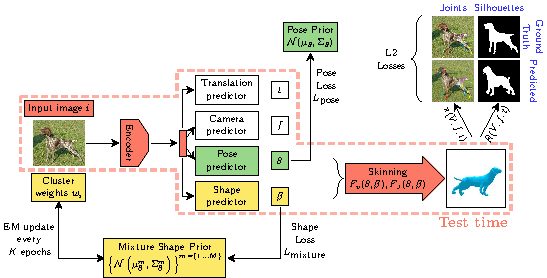
\includegraphics[width=\textwidth]{OllieFigs/system_overview_cr.pdf}
    \caption{Our method consists of (1) a deep CNN encoder which condenses the input image into a feature vector (2) a set of prediction heads which generate SMBLD parameters for shape $\beta$, pose $\theta$, camera focal length $f$ and translation $t$ (3) skinning functions $F_v$ and $F_J$ which construct the mesh from a set of parameters, and (4) loss functions which minimise the error between projected and ground truth joints and silhouettes. Finally, we incorporate a mixture shape prior (5) which regularises the predicted 3D shape and is iteratively updated during training using expectation maximisation. At test time, our system (1) condenses the input image, (2) generates the SMBLD parameters and (3) constructs the mesh.}
    \label{fig:sys_overview_train_sup}
\end{figure*}
    
\def\smalrestT{\bar{T}}
\def\smalrestJ{J}
\def\smalbweightsW{\mathcal{W}}

\def\smalrestv#1#2{\bar{#1_{#2}}}
\def\smalbweightw{w}

\def\poseele#1{\omega_{#1}}
\def\poseelenorm#1{\bar{\omega_{#1}}}

\newcommand{\bigzero}{\mbox{\normalfont\Large\bfseries 0}}
\newcommand{\bigone}{\mbox{\normalfont\Large\bfseries 1}}
\newcommand{\rvline}{\hspace*{-\arraycolsep}\vline\hspace*{-\arraycolsep}}


\section{Building SMBLD: a new parametric dog model}

% Explain why the SMAL parameteric model is unsuitable for the dog category.

At the heart of the method is a parametric mesh representation of a 3D animal, which is based on the Skinned Multi-Animal Linear (SMAL) model proposed by Zuffi et al.~\cite{zuffi2017menagerie}. As discussed in \Cref{chap:cgas}, SMAL is a deformable 3D quadruped mesh parameterized by shape and pose. The \emph{shape}~$\shape \in \R\nshape$ parameters are PCA coefficients of an undeformed template mesh with limbs in default position. The \emph{pose}~$\pose \in \R\npose$ parameters meanwhile govern the joint angle rotations ($35 \times 3$ Rodrigues parameters) which effect the articulated limb movement. 

% The SMAL generator function can therefore be viewed supplying a set of triangles and a function 
% \begin{equation}
% \verts(\pose, \shape) : \R \npose \times \R \nshape \mapsto \RR 3 \nverts
% \end{equation}
% which generates the set of 3D model vertex positions $\verts(\pose, \shape) \in \RR{3889}{3}$ for the given pose and shape. Also required are a set of position parameters $\posn$ which govern the global orientation and translation of the model. The following represents a 3D model of given pose and shape transformed to its 3D position
% \begin{equation}
%     \posn * \verts(\pose, \shape)
% \end{equation}    

% In addition, the 3D joints locations on the SMAL modal are obtained from the output vertex set by post-multiplying by a $\nverts \times \njoints$ matrix $\jointselect$.  The $j^{\text{th}}$ column of~$\jointselect$ defines the 3D position of joint~$j$ as a linear combination of the vertices
% \begin{equation}
% J(\pose, \shape, \posn) := \posn * \verts(\pose, \shape) \jointselect
% \end{equation}

First, it is important to give a detailed description of the SMAL generator function, which is later augmented with scale parameters to improve model flexibility. 
\begin{equation}
    v(\pose,\shape) = W(T_{P}(\pose, \shape), J(\shape), \pose, \smalbweightsW)
\end{equation}
\begin{equation}
    T_{P}(\pose,\shape) = \smalrestT + B_{S}(\shape) + B_{P}(\pose)
\end{equation}

Here, SMAL relies on a standard linear blend skinning (LBS) formulation to return a set of posed vertices from SMAL template vertices in rest pose $\smalrestT$, SMAL 3D joint locations $\smalrestJ$, a pose vector $\pose$ and blend weights $\smalbweightsW$
\begin{equation}
    W(\smalrestT,\smalrestJ,\pose,\smalbweightsW) : \mathbb{R}^{3N \times 3K \times |\pose| \times |\smalbweightsW|} \mapsto \R{3N}
\end{equation}

The rest pose mesh $T_{P}(\pose,\shape) \in \RR{3889}{3}$ is constructed from the SMAL template vertices $\smalrestT$ and additive vertex offsets $B_{S}(\shape)$ and $B_{P}(\pose) \in \RR{3889}{3}$. These are referred to as shape and pose blend shapes respectively. Note that despite being a function of pose, $B_{P}(\pose)$ still represents a shape modification. This is often referred to as a \emph{corrective} offset, fixing artefacts common to linear blend skinning, often by fat. The pose vector $\pose = \left[\poseele{0}^{T},\dots,\poseele{\njoints}^{T}\right]^{T}$ contains 3 parameters for each joint. Each element $\poseele{j} \in \R{3}$ denotes the axis-angle representation of the relative rotation of each part $j$ with respect to its parent in the kinematic tree. The local $3 \times 3$ rotation matrix corresponding to a joint $j$ is denoted $\exp(\poseele{j})$ and is obtained from axis angle representation using the \emph{Rodrigues formula}
\begin{equation}
    \exp(\poseele{j}) = \mathcal{I} + \hat{\poseelenorm{j}}\sin(||\poseele{j}||) + \hat{\poseelenorm{j}}^{2}\cos(||\poseele{j}||)
\end{equation}
where $\hat{\poseelenorm{j}}$ is the skew symmetric matrix of the 3-vector $\bar{\omega} = \frac{\omega}{||\omega||}$ representing the unit norm axis of rotation. $\mathcal{I}$ is the $3 \times 3$ identity matrix.

The linear blend skinning function (LBS) is then used to articulated the rest pose mesh $T_{P}(\pose,\shape)$. Let $t_{i} = \smalrestv{t}{i} + b_{S,i}(\shape) + b_{P,i}(\pose) \in T_{P}(\pose,\shape)$ be a \emph{shaped} vertex in rest pose where $b_{S,i}(\shape)$ and $b_{P, i}(\pose)$ denotes the same vertex in $B_{S}(\shape)$ and $B_{P}(\pose)$ respectively. The transformation to obtain a \emph{posed} vertex $t'_{i}$ is then
\begin{equation}
    t'_{i} = \sum_{k=1}^{K} \smalbweightw_{k,i} G_{k}'(\pose,\smalrestJ)t_{i}
\end{equation}
\begin{equation}
    G'_{k}(\pose,\smalrestJ) = G_{k}(\pose,\smalrestJ) G_{k}(\pose^{*},\smalrestJ)^{-1}
\end{equation}
\begin{equation}\label{eqt:kintree_prods}
    G_{k}(\pose,\smalrestJ) = \prod_{j \in A(k)} 
    \begin{pmatrix}
        \exp(\poseele{j})
        & \rvline 
        & j_{j} \\
    \hline
        \bigzero
        & \rvline 
        & \bigone
    \end{pmatrix}
\end{equation}
Here, $\smalbweightw_{k,i}$ is an element of the blend weight matrix $\smalbweightsW$, representing how much the rotation of part $k$ effects the vertex $i$, $\exp(\poseele{j})$ is the local $3 \times 3$ rotation matrix corresponding to joint $j$, $G(\pose,\smalrestJ)$ is the world transformation of joint $k$, and $G'(\pose,\smalrestJ)$ is the same transformation after removing the transformation due to the rest pose $\pose^{*}$. Each $3$-element vector in $J$ corresponding to a single joint center $j$, is denoted $j_{j}$ . Finally, $A(k)$ denotes the ordered set of joint ancestors of joint $k$.

% Using this definition, a vertex $\smalrestv{t'}{i}$ is transformed according to 
% \begin{equation}
%     \smalrestv{t'}{i} = \sum_{k=1}^{K} \smalbweightw_{k,i} G'(\pose,J(\shape))(\smalrestv{t'}{i} + b_{S,i}(\shape) + b_{P,i}(\pose))
% \end{equation}

% where $b_{S,i}(\shape)$ and $b_{P, i}(\pose)$ are vertices in $B_{S}(\shape)$ and $B_{P}(\pose)$ respectively and represent the shape and pose blend shape offsets for the vertex $\smalrestv{t'}{i}$.

\subsubsection{Shape blend shapes}

Shape blend shapes are applied to the SMAL rest model to smoothly modify the mesh's body proportions. This has the effect of appearing to alter the animal category. The body shapes are globally represented by a linear function $B_{S}$

\begin{equation}\label{eqt:shapeblendshapes}
    B_{S}(\shape;\mathcal{S}) = \sum_{n=1}^{|\shape|}\shape_{n}S_{n}
\end{equation}
where $\shape \in \R{41}$ is a vector of linear shape coefficients and $S_{n}$ represents the orthnormal principle components of shape displacements, learned from the registered training scans. 

% SHOW THIS?

\subsubsection{Pose blend shapes}

Let $R: \R{|\pose|} \mapsto \R{9K}$ be a function which maps the pose vector $\pose$ to a vector of concatenated part relative rotation matrices $\exp(\pose)$. Given the SMAL model contains $33$ joints, $R(\pose)$ is a vector of length $33 \times 9 = 297$. Since elements of $R(\pose)$ comprise sine and cosine functions of the input pose vector, $R(\pose)$ is therefore non-linear with respect to $\pose$.

The pose blend shapes are defined to be linear in $R^{*}(\pose) = (R(\pose) - R(\pose^{*}))$ where $\pose^{*}$ denotes the rest pose. Letting $R_{n}(\pose)$ denote the $n^{th}$ element of $R(\pose)$, the vertex deviations from the rest template are
\begin{equation}
    B_{P}(\pose;\mathcal{P}) = \sum_{n=1}^{9K} (R_{n}(\pose) - R_{n}(\pose^{*}))P_{n}
\end{equation}

An important observation is that by subtracting the rest pose $R(\pose^{*})$, the contribution of the pose blend shape is zero when the model is in the rest pose.

\subsubsection{Joint locations}

Differing animal body shapes have an effect on the 3D joint locations. 

\begin{equation}
    J(\shape; J, \smalrestT, \mathcal{S}) = \mathcal{J}(\smalrestT + B_{S}(\shape; \mathcal{S}))
\end{equation}
where $\mathcal{J}$ is a matrix that transforms rest vertices into rest joints.

\subsubsection{Complete formulation}

The complete formulation is therefore given as

\begin{equation}
    v(\pose,\shape;\smalrestT,\smalbweightsW,\mathcal{S},\mathcal{J},\mathcal{P}) = W\big(T_{P}(\pose,\shape; \smalrestT,\mathcal{S},\mathcal{P}), J(\shape; \mathcal{J}, \smalrestT, \mathcal{S}), \pose, \smalbweightsW\big)
\end{equation}

% model consists of a linear blend skinning function $F_{v}: (\pose, \shape) \mapsto V$, which generates a set of vertex positions $V \in \RR{3889}{3}$, and a joint function $F_{J}: (\pose, \shape) \mapsto J$, which generates a set of joint positions $J \in \RR{35}{3}$.

% TODO: Use consistent notation!
% This section provides a formal definition for the deformable 3D model that is used to generate synthetic training data and in the model fitting stage to obtain the final mesh. Our system assumes a deformable 3D model such as SMAL~\cite{zuffi2017menagerie} which parametrizes a 3D mesh as a function of {\em pose} parameters~$\pose \in \R\npose$ (e.g.\ joint angles) and {\em shape} parameters~$\shape \in \R\nshape$. 
% As discussed in \Cref{chap:relwork}, a 3D mesh is an array of vertices $\verts \in \RR 3\nverts$ (the vertices are columns of a $3 \times \nverts$ matrix) and a set of triangles represented as integer triples $(i,j,k)$, which are indices into the vertex array.
% A deformable model such as SMAL may be viewed as supplying a set of triangles, and a function
% \begin{equation}
% \verts(\pose, \shape) : \R \npose \times \R \nshape \mapsto \RR 3 \nverts
% \end{equation}
% which generates the 3D model for a given pose and shape.
% The mesh topology (i.e.~the triangle vertex indices) is provided by the deformable model, and is the same for all shapes and poses we consider, so in the sequel a mesh will be defined only by the 3D positions of its vertices.

% In any given image, the model's 3D {\em position} (i.e.\ translation and orientation) is also unknown, and will be represented by a parametrization $\posn$ which may be for example translation as a 3-vector and rotation in axis angle form. Application of such a transformation to a $3\times\nverts$ matrix will be denoted by $*$, so that 
% \begin{equation}
% \posn * \verts(\pose, \shape)
% \end{equation}
% represents a 3D model of given pose and shape transformed to its 3D position.


\subsection{Introducing scale parameters}

While SMAL has been shown to adequately represent a variety of quadruped types, the modes of dog shape variation are poorly captured by the current model. This is unsurprising, since SMAL used only four dogs in its construction. This limitation is overcome using a simple but effective method that improves the model's representational power over this particularly diverse animal category. The set of shape parameters $\beta$ are augmented with an additional set $\scale$ which independently scale parts of the mesh. For each model joint, parameters ${\scale_x,\scale_y,\scale_z}$ are defined which apply a local scaling of the mesh along the local coordinate $x, y, z$ axes, before pose is applied. 

A simple method for adding scaling parameters is to apply a transformation to the rotation matrices for each joint. \Cref{eqt:kintree_prods} then becomes
\begin{equation}
    G_{k}(\pose,\smalrestJ) = \prod_{j \in A(k)} 
    \begin{pmatrix}
        Q_{j} \exp(\poseele{j})
        & \rvline 
        & j_{j} \\
    \hline
        \bigzero
        & \rvline 
        & \bigone
    \end{pmatrix}
\end{equation}

where the matrix
\begin{equation}
    Q_{j} = \begin{pmatrix}
        \scale_{j,x} & 0 & 0 \\
        0 & \scale_{j,y} & 0 \\
        0 & 0 & \scale_{j,z}
    \end{pmatrix}
\end{equation}

Unfortunately, this formulation causes challenges should a user wish to scale a mesh subpart along the kinematic tree. While it is natural for joint \emph{rotations} to be compositionally applied along the kinematic tree (mirroring the effect of skeletal limb motion) this does not follow for scaling parameters. For example, it is common for a user to apply scaling to a subpart which does not necessarily affect subsequent parts. With the formulation at present, it would be the responsibility of the user to ``undo'' scaling for the remaining tree, requiring them to be aware of the kinematic tree index ordering. This is seen as suboptimal behaviour, so the following formulation is preferred, defining \emph{absolute} scale parameters that do not propagate their effect. Taking advantage of the hierarchical ordering of the kinematic tree for joint $k$, $A(k) = \left[A(k)_{0}, A(k)_{1}, \dots, k\right]$ are joints along the tree. Therefore, the absolute scaling matrix is given by
\begin{equation}
    G_{k}(\pose,\smalrestJ) = 
    \begin{pmatrix}
        \exp(\poseele{A(k,0)}) Q_{A(k,0)}
        & \rvline 
        & j_{A(k,0)} \\
    \hline
        \bigzero
        & \rvline 
        & \bigone
    \end{pmatrix}
    \prod_{j \in \left[A(k)_{1}, \dots, k \right]}
        \begin{pmatrix}
            Q_{j-1}^{-1} \exp(\poseele{j}) Q_{j}
            & \rvline 
            & j_{j} \\
        \hline
            \bigzero
            & \rvline 
            & \bigone
        \end{pmatrix}
\end{equation}
Note that $Q_{j-1}$ refers to the parent scaling matrix of joint $j$. Note that the scale parameters in this formulation determine only the scale for the particular subpart by undoing that of the parent.

\subsection{Sharing scale parameters}

Allowing each joint to scale entirely independently can however lead to unrealistic deformations. To overcome this, scale parameters are shared between multiple joints which are physiologically related and would naturally scale together. For example, the $y$-scaling for the four legs (which governs the length) is controlled by only a single parameter. The new Skinned Multi-Breed Linear Model for Dogs (SMBLD) is therefore adapted from SMAL by adding $6$ scale parameters to the existing set of shape parameters. Figure~\ref{fig:shape_variation} shows how introducing scale parameters increases the flexibility of the SMAL model. The next task is to learn an prior (with which to initialize the later EM process) that covers these new scale parameters. 

\begin{figure*}[t!]
    \centering
    % \includegraphics[width=0.23\linewidth]{OllieFigs/mean.png}
    % \includegraphics[width=0.23\linewidth]{OllieFigs/leg_lengthen.png}
    % \includegraphics[width=0.23\linewidth]{OllieFigs/tail_shorten.png}
    % \includegraphics[width=0.23\linewidth]{OllieFigs/tail_puff.png}
    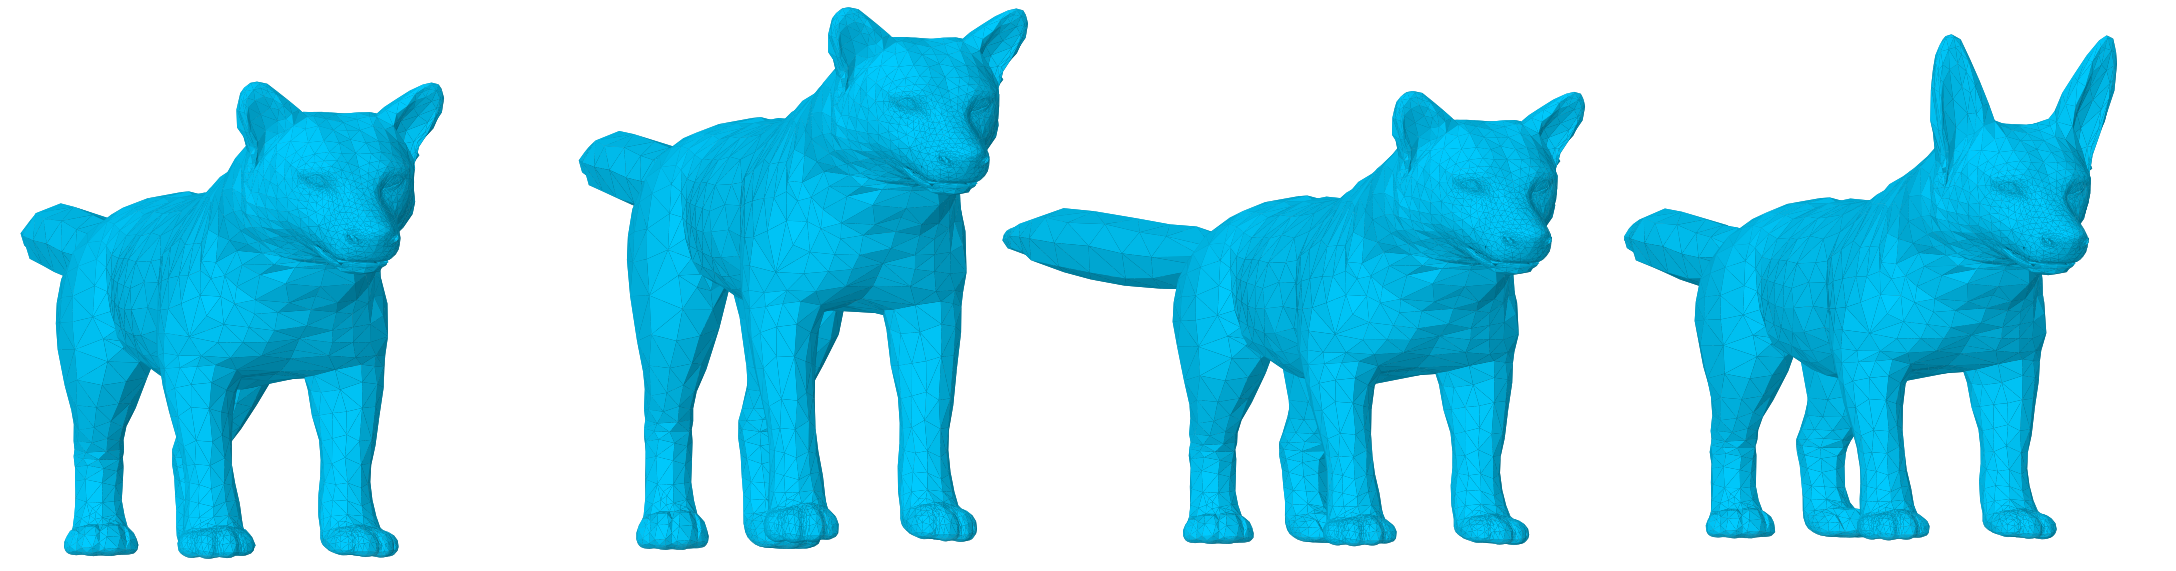
\includegraphics[width=.95\linewidth]{OllieFigs/all_shapevar.png}
    \caption{\textbf{Effect of varying SMBLD scale parameters}. 
    \emph{From left to right}: 
    Mean SMBLD model, 
    25\% leg elongation,
    50\% tail elongation,
    50\% ear elongation.}
    \label{fig:shape_variation}
\end{figure*}

\subsection{Initializing a dog shape/scale prior}

The SMBLD shape prior is initialized by fitting the model to a set of $13$ artist-designed 3D dog meshes, downloaded from the internet and are similar in style to the SMAL toys. While the collection does offer a few more examples of dogs than used in the original SMAL set, the models still lack realism and are very constrained when compared to the 120 different breeds represented in the later test set. An energy minimization process is used to align the SMBLD vertices to each scan, in order to obtain a set of shape $\shape$, pose $\pose$ and $\scale$ parameters. 

\subsubsection{Fitting SMBLD to 3D scans}

Recall that SMBLD's shape $\shape$ and $\pose$ parameters are exactly as defined in SMAL, meaning there is no need to relearn (or adapt) the blend shape data $\mathcal{P}, \mathcal{S}$ or joint selectors $\jointselect$. The scale $\scale$ parameters, however, are new to SMBLD. The goal of this section is to learn a new 3D prior over both shape and scale parameters to initialize the prior refined during the WLDO training loop.

Note that fitting SMBLD to 3D scans emits much simpler optimization in comparison to 2D images, since the complete 3D information of the target mesh is available. In addition, the target meshes are not particularly detailed and are already aligned in the canonical T-pose, so we avoid need for a complex alignment technique as discussed in \Cref{chap:cgas}. 

% \def\seq#1#2#3#4{\left[{#1_{#2}}\right]_{#2=#3}^{#4}}

An energy minimization process is used to align the SMBLD mesh $v(\pose,\shape)$ to each of the 3D scans $\seq{(V, T)}{i}{1}{N}$ subject to smoothing regularizers. The following energy formulation is minimized using stochastic gradient descent (SGD) with learning rate $1.0e^{-4}$ for $1000$ iterations

\begin{equation}
    \E{opt} = \E{chamfer} + \E{laplacian} + \E{edge} + \E{normal}
\end{equation}
where each of these terms has a scalar weight $\lambda$. Here, $\W{chamfer}=\W{edge}=1.0$, $\W{normal}=0.01$ and $\W{laplacian}=0.1$. Further details on the specific energy terms are now provided.

\ss{Chamfer energy.} Chamfer energy measures the average distance between vertices of the SMBLD mesh $V = v(\pose,\shape)$ and the target mesh vertices $V'$. Let $V_{P} = \seq{v}{i}{1}{p}$ and $V'_{P} = \seq{v'}{i}{1}{p}$ be random $p$-subsets of $V$ and $V'$ respectively. The chamfer energy is then
\begin{equation}
        \E{chamfer}(V_{P}, V'_{P}) = \frac{1}{p} \sum_{i=1}^{p} \min_{j}  \left | v_{i} - v'_{j} \right |
\end{equation}

\ss{Uniform laplacian energy.} 

% TODO: AWF, ask about this function

% https://pytorch3d.readthedocs.io/en/latest/modules/loss.html
% [1] Desbrun et al, “Implicit fairing of irregular meshes using diffusion and curvature flow”, SIGGRAPH 1999.
% [2] Nealan et al, “Laplacian Mesh Optimization”, Graphite 2006.

The SMAL mesh can be viewed as $M = (v(\pose,\shape), T)$ where the vertices are given by the generator function above and the triangulation is fixed. The uniform Laplacian matrix $L \in \RR{N}{N}$ is defined as $LV = w_{i} \sum_{j} (v_{j} - v_{i})$ where $w_{ij} = 1 / |S_{i}|$ and $S_{i}$ is the set of neighbouring vertices to $i$. Note that $LV_{i}$ points to the centroid of the neighbouring vertices. The energy formulation is then

\begin{equation}
    \E{laplacian} = \sum_{i} w_{i} \sum_{j} (v_{j} - v_{i})
\end{equation}

%$LV_{i} = \sum_{j}w_{ij} (v_{j} - v_{i})$. For the uniform case, used here, $w_{ij} = 1 / |S_{i}|$ where $S_{i}$ is the set of neighbouring vertices to $i$. 


\ss{Edge energy.} 

This energy is equal to the average edge length across the mesh, and is used to encourage uniform distribution of vertices. Let $E = \SET{(i,j)}{$v_{i}, v_{j} \in V$ are adjacent vertices}$, then
\begin{equation}
    \E{edge} = \frac{1}{|E|} \sum_{(i,j) \in E} || v_{j} - v_{i} ||
\end{equation}

\ss{Normal energy.} 

% TODO; define normal, cross product between two triangle edges
Normal energy is a measure of the average normal consistency between adjacent triangles. For two triangles $t_{i}, t_{j} \in T$ in SMAL's fixed triangle set, let $n_{i}, n_{j}$ be the respective normals. Recall that $n = (v_{1} - v_{0}) \cdot (v_{2} - v_{0})$. Then normal consistency is defined by
\begin{equation}
    \E{normal} = 1 - \frac{n_{i} \cdot n_{j}}{\left|n_{i}\right|\left|n_{j}\right|}
\end{equation}

% \begin{equation}
%     \E{normal} = 1 - \frac{\mathbf{n_0} \cdot \mathbf{n_1}}{\left|\mathbf{n_0}\right|\left|\mathbf{n_1}\right|}
% \end{equation}

% This energy promotes consistency between adjacent faces. It is a measure of the average normal consistency between adjacent faces. For two faces with normals $\mathbf{n_0}$ and $\mathbf{n_1}$, the normal consistency is $1 - \frac{\mathbf{n_0} \cdot \mathbf{n_1}}{\left|\mathbf{n_0}\right|\left|\mathbf{n_1}\right|}$.

At the end of this process, we have a collection of fits $\left|(\pose,\shape)\right|_{\{i=1,...13\}}$ from which we can learn our unimodal pose and shape priors. As discussed, we evenutally use this unimodal shape prior to initialize our mixture shape prior, which is tuned with the expectation-maximization step in the training loop.

\subsubsection{Learning a unimodal prior}

Recall that the SMAL body shapes are represented by the linear function in \Cref{eqt:shapeblendshapes}. In this formulation, the matrix $S_{n}$ represents the orthonormal principal components of shape displacements. A consquence of the PCA construction is that the features in $\nshape$-dimensional parameter space (as they are linear combinations of the original features) are normally distributed with mean $\shapemu$ and covariance matrices $\shapecov$. With this construction, a likelihood function measures the probability of a given shape vector $\shape \in \R{\nshape}$

\begin{equation}
    \mathbb{P}_{\shape}(\shape) = (2\pi)^{-\frac{\nshape}{2}}\det(\shapecov)^{-\frac{1}{2}}e^{-\frac{1}{2}(\shape-\shapemu)^{T}\shapecov^{-1}(\shape-\shapemu)}
\end{equation}

For problems which aim to optimize $\shape$ as a free variable, the 3D shape prior is obtained by maximizing $\mathbb{P}_{\shape}(\shape)$ or equivalently, by minimizing the negative log likelihood

\begin{equation}
     -\ln\left[\mathbb{P}_{\shape}(\shape)\right] = -\frac{1}{2}\left[\ln\det(\shapecov) + \nshape\ln(2\pi) +  (\shape - \shapemu)^T\Sigma^{-1}(\shape-\shapemu)\right]
\end{equation}
Finally, terms with no dependency on $\shape$ can be dropped since they remain constant during the optimization. This reduces the formulation of the loss as the Mahalanobis distance of $\shapemu$

\begin{equation}
    \L{shape}(\shape;\shapemu,\shapecov) = (\shape - \shapemu)^{T}\shapecov^{-1}(\shape - \shapemu)
\end{equation}

A similar construction applies to the scale parameters $\scale$ with means and covariances computed from the 13 training scans. The scale loss function is therefore given as

\begin{equation}
    \L{scale}(\scale;\scalemu,\scalecov)= (\scale - \scalemu)^{T}\scalecov^{-1}(\scale - \scalemu)
\end{equation}

Continuing from here, it is convenient to group shape and scale parameters into a new shape-scale variable $\shapescale$ and the loss function can be grouped as follows
\begin{equation}
    \L{shape-scale}(\shapescale=\left[\shape,\scale\right];\shapescalemu=\left[\shapemu,\scalemu\right],\shapescalecov=\left[\shapecov,\scalecov\right]) = \L{shape}(\shape;\shapemu,\shapecov) + \L{scale}(\scale;\scalemu,\scalecov)
\end{equation}

% END PRELIMINARIES

% We have already seeen this formulation in Chapter 4.

% \subsubsection{Learning an improved prior via 3D model fitting}

% Recall that SMBLD is adapted from the SMAL~\cite{zuffi2017menagerie} deformable animal mesh, by including limb scaling parameters. A new shape prior is learnt by fitting this new SMBLD model, which comprises parameters for pose $\pose$ and shape $\beta$ (the latter of which now includes scaling parameters $\kappa$).

\subsubsection{Extending to a multimodal prior}

\def\imgweight{w}

So far, a shape-scale prior has been introduced based on a unimodal, multivariate Gaussian with mean $\shapescalemu$ and covariance matrix $\shapescalecov$. However, enforcing this throughout training tends to result in model predictions that appear similar in 3D shape, even when tested on dog images of different breeds. Diversity is improved among predicted 3D dog shapes by extending the above formulation to a Mixture of $M$ Gaussians prior.

Here, $\shapescalemu^{m}$, $\shapescalecov^{m}$ and $\shapescalepi^{m}$ are the mean, covariance and mixture weight respectively for Gaussian component 
$m$. For each component, the mean is sampled from the existing unimodal prior and the covariance is set equal to the unimodal prior i.e. $\shapescalecov^{m} := \shapescalecov$. All mixture weights are initially set to $\frac{1}{M}$.

The mixture shape loss is given as:
\begin{align}
    \L{mixture}(\shapescale_{i}; \shapescalemu, \shapescalecov, \shapescalepi)
    =&
    \sum_{m=1}^M \shapepi^{m} \left[\L{shape-scale}(\shapescale_{i}; \shapescalemu^{m}, \shapescalecov^{m})\right]
\end{align}



% \section{Learning mixture shape prior.}
% This section contains additional detail for how we learn our mixture shape prior, using expectation maximization in-the-loop.


% Way more here, and include exampels
\section{End-to-end dog reconstruction from monocular images} 

This section describes a technique for reconstructing a 3D dog mesh from a single, monocular image. This is achieved using an end-to-end convolutional neural network, which predicts pose $\pose$ and shape-scale $\shapescale$ for the SMBLD morphable dog model, translation and orientation $\posn$ and focal length $f$ for a perspective camera $\proj_{f}$. A complete overview of the proposed system is shown in Figure~\ref{fig:sys_overview_train_sup}.

% the model's 3D {\em position} (i.e.\ translation and orientation) is also unknown, and will be represented by a parametrization $\posn$ which may be for example translation as a 3-vector and rotation in axis angle form. Application of such a transformation to a $3\times\nverts$ matrix will be denoted by $*$, so that 
% \begin{equation}
% \posn * \verts(\pose, \shape)
% \end{equation}

\subsection{Model architecture}

%extended with convolutional layer and an fully-connected layer 
The network architecture for WLDO is inspired by the model of 3D-Safari~\cite{Zuffi19Safari}. Given an input image cropped to (224, 224), a Resnet-50~\cite{he2016deep} backbone network is applied in order to encode a 1024-dimensional feature map. These features are passed through various linear prediction heads to produce the required parameters. The pose, translation and camera prediction modules follow the design of 3D-Safari, but we describe the differences in our shape-scale module.

\ss{Pose, translation and camera prediction.}
These modules are independent multi-layer perceptrons which map the above features to the various parameter types. As with 3D-Safari, two linear layers are used to map to a set of $35 \times 3$ 3D pose parameters (three parameters for each joint in the SMBLD kinematic tree and three parameters for the model orientation) given in Rodrigues form. The translation component of the SMBLD model is predicted with two linear layers that predict translation in the camera frame $\trans_{x,y}$ and depth $\trans_{z}$ independently. The camera prediction layer predicts the focal length of the perspective camera. Note that while this parameter is theoretically unnecessary since model depth is already predicted, as in the original 3D-Safari implementation, including the parameter produces empirally better fits. The camera focal length is obtained as $f = f_{0} + f_{1}x$ where $x$ is predicted by the network and $f_{0} = f_{1} = 2700$.

\ss{Shape and scale prediction.}

Unlike 3D-Safari, WLDO predicts a set of shape and scale parameters rather than vertex offsets. Separate predictions heads are used to predict 20 shape parameters $\shape$ and the new scale parameters $\kappa$. The scale parameters are obtained as $\scale = \exp{x}$ where $x$ are the network predictions, as predicting log scale helps stabilise early training and conveniently guarantees non-negative values for scale.

\subsection{Training losses}

A typical approach for training such an end-to-end system would be to supervise the prediction of $(\pose, \shapescale, \posn, \f)$ with 3D ground truth annotations~\cite{kolotouros19learning,kanazawa18end-to-end,pavlakos18learning}. However, building a suitable 3D annotation dataset would require an experienced graphics artist to design an accurate ground truth mesh for each of 20,520 StanfordExtra dog images, a prohibitive expense.

Instead, WLDO relies on \emph{weak 2D supervision} provided by 2D keypoints and silhouette segmentations to guide network training. These data sources are significantly cheaper to obtain than 3D models.

The remainder of this section describes the set of losses used to supervise the network at train time.

\ss{Joint reprojection.}
As in \Cref{chap:cgas}, the joint projection loss $\L{joints}$ promotes accurate limb positioning by comparing the projected model joints to the ground truth annotations $X^{*}$. To achieve this, the SMBLD generator function processes the network's pose $\pose$ and shape-scale $\shapescale$ parameters to generate a set of 3D joint positions which are translated and orientated with $\posn$. The joint positions are then projected to the image plane using the camera parameters. The joint loss $\L{joints}$ is given by the $\ell_2$ error between the ground truth and projected joints:

\begin{equation}
\L{joints}(\pose, \shapescale, \posn, \f; X^{*}) = \lVert X^{*} - \proj_{f}(\posn * \verts(\pose, \shapescale) \jointselect) \rVert_{2}
\end{equation}

Note that many of the training images contain significant occlusion, so $X^{*}$ contains many invisible joints. This is handled by masking $\L{joints}$ so that invisible joints do not contributing to the loss.

\ss{Silhouette loss.}
The silhouette loss $\L{sil}$ is used to promote shape alignment between the SMBLD dog mesh and the input dog. In order to compute the silhouette loss, a rendering function $R\bigl(\posn * \verts(\pose, \shapescale)\bigr) \in \mathbb{B}^{W\times H}$ projects the SMBLD mesh to produce a binary segmentation mask. In order to allow derivatives to be propagated, $R$ is implemented using the differentiable Neural Mesh Renderer~\cite{kato2018renderer}. The loss is computed as the $\ell_2$ difference between a projected silhouette and the ground truth mask $S$:

\begin{equation}
\L{sil}(\pose, \shapescale, \posn, \f; S) = \lVert S - R\bigl(\posn * \verts(\pose, \shapescale)\bigr) \rVert_{2}
\end{equation}

% The model is also assumed to be supplied with a rendering function $R$ which takes a vertex array in camera coordinates, and generates a 2D binary image of the model silhouette.  That is,
% \begin{equation} \label{eq:render_sil}
% R\bigl(\posn * \verts(\pose, \shape)\bigr) \in \mathbb{B}^{W\times H}
% \end{equation}
% for an image resolution of $W \times H$. 

\ss{Pose prior.}
In the absence of 3D ground truth training data, priors are obtained from artist graphics models in order to encourage realism in the network predictions. The pose prior is modelled as a multivariate Gaussian prior consisting of mean $\mu_{\pose}$ and a covariance matrix $\Sigma_{\pose}$. The loss is given as the log likelihood of a given shape or pose vector under these distributions, which corresponds to the Mahalanobis distance between the predicted parameters and their corresponding means:
\begin{align}
    \L{pose}(\pose; \mu_{\pose}, \Sigma_{\pose}) &= (\pose - \mu_{\pose})^T \Sigma_{\pose}^{-1} (\pose - \mu_{\pose})\\
\end{align}
Unlike previous work, there is no need to use a loss for penalizing pose parameters if they exceed manually specified joint angle limits. It is suspected that that the WLDo network learns this regularization naturally by training on the large dataset.

\ss{Shape-scale prior.}
As discussed in the previous section, the shape prior is modelled as a mixture of $M$ Gaussians. 
Recall that $\shapescalemu^{m}$, $\shapescalecov^{m}$ and $\shapescalepi^{m}$ are the mean, covariance and mixture weight respectively for each Gaussian component 
$m$. From before, the mixture shape loss is given as:
\begin{align}
    \L{mixture}(\shapescale_{i}; \shapescalemu, \shapescalecov, \shapescalepi)
    =&
    \sum_{m=1}^M \shapepi^{m} \left[\L{shape-scale}(\shapescale_{i}; \shapescalemu^{m}, \shapescalecov^{m})\right]
\end{align}

\section{Expectation Maximization in the Loop}

% Using a unimodal prior tends to result in predictions which look relatively similar in shape. To promote diversity among predicted 3D dog shapes, our method extends the formulation above to incorporate a mixture of Gaussians prior. We represent the mixture as a set of $M$ Gaussians, whose means are initialized by drawing samples from our existing prior:

% \begin{align}
%     \mu_{\shape}^{m} &\sim N(\mu_{\shape}, \Sigma_{\shape}) \\
%     \Sigma_{\shape}^{m} &:= \Sigma_{\shape}
% \end{align}

% We assign each training image $i$ with a set of mixture weights $\{w_{i}^{1}, \dots w_{i}^{M}\}$, where initially $w_{i}^{m} := \frac{1}{M}.$

% We can then apply the following mixture shape loss:

% \begin{equation}
%     L_{mixture}=\sum_{m=1}^M w_{i}^{m}L_{shape}(\shape_{i}, \mu_{\shape}^{m}, \Sigma_{\shape}^{m})
% \end{equation}

% In order to allow our mixture prior to learn ``in-the-loop" from the available training data, we apply expectation maximization every $k$ epochs during training. This step recomputes the means and variances for each mixture component based on the observed shapes in the training set, and updates the per-image mixture weights:

% \begin{align}
%     \mu_{\shape}^{m} :=& \mathrm{E}_{i}[\beta_{i}W_{i}^{m}]\\
%     \Sigma_{\shape}^{m} :=& \mathrm{Cov}_{i}[\beta_{i}W_{i}^{m}, \beta_{i}W_{i}^{m}]\\
%     w_{i}^{m} :=& \frac{L_{shape}(\shape_{i}, \mu_{\shape}^{m}, \Sigma_{\shape}^{m})}{\sum_{m'}^{M}L_{shape}(\shape_{i}, \mu_{\shape}^{m'}, \Sigma_{\shape}^{m'})}
% \end{align}


% \section{Attempt 2}

As previously discussed, the parameters for the mixture shape-scale prior are initialized using artist data which results in a prior that poorly represents the diverse shapes present in the real dog dataset. A key contribution presented in this chapter is the introduction of a procedure based on Expectation Maximization which gradually improves the representational power of the shape-scale prior by learning from monouclar images of in-the-wild dogs and their respective 2D training labels.

% \subsection{Assigning image weights}

\def\imgweight#1#2{w_{#1}^{#2}}

Firstly, each training image is assigned a set of latent variables $\{\imgweight{i}{1}, \dots, \imgweight{i}{M}\}$ which encode the likelihood that the dog in image~$i$ was generated according to each shape-scale component~$m \in \{1,\dots,M\}$. 

Expectation Maximization (EM) is then used to regularly update these image weights, as well as the parameters for the mixture $(\shapescalemu^{m},\shapescalecov^{m},\shapescalepi^{m})_{i=1}^{M}$. During the training loop of the 3D reconstruction network, these parameters are tuned according to alternating expectation (`E-') and maximization (`M-') steps which are described below:

% TODO - add me!
% Each training image $i$ is assigned a set of latent variables encoding the probability of the dog shape in image~$i$ being generated by component~$m$. 

% This is addressed by proposing to recover the latent variables $w_{i}^{m}$ and parameters $\shapescalemu^{m}$, $\shapescalecov^{m}$ and $\shapescalepi^{m}$ ($\mu_{\shape}^{m}$, $\Sigma_{\shape}^{m}$ and $\Pi_{\shape}^{m}$) of our 3D shape prior by learning from monocular images of in-the-wild dogs and their 2D training labels in our training dataset.

% We achieve this using Expectation Maximization (EM), which regularly updates the means and variances for each mixture component and per-image mixture weights based on the observed shapes in the training set. While training our 3D reconstruction network, we progressively update our shape mixture model with an alternating `E' step and `M' step described below:

\subsection{Expectation Maximization update steps}

\subsubsection{The `E' Step.}
The `E' step computes the expected value of the image weights~$w_{i}^{m}$ 
assuming fixed $(\shapescalemu^{m},\shapescalecov^{m},\shapescalepi^{m})$ for all $i \in \{1,\dots,N\}, m \in \{1,\dots,M\}$.

The update equation for an image $i$ with latest scale-shape prediction $\shapescale_{i}$ and cluster $m$ with parameters $(\shapescalemu^{m},\shapescalecov^{m},\shapescalepi^{m})$ 
is given as:

\begin{align}
    \imgweight{i}{m}
    :=& 
    \frac{
        \mathcal{N}(\shapescale_{i} | \shapescalemu^{m},\shapescalecov^{m})\shapescalepi^{m}
    }
    {
        \sum_{m'=1}^{M}
        \mathcal{N}(\shapescale_{i} | \shapescalemu^{m'},\shapescalecov^{m'})\shapescalepi^{m'}
    }
\end{align}

To improve numerical stability, this is formulated using the log-sum-exp trick:

\begin{align}
    \log{\imgweight{i}{m}}
    :=& 
    \frac{
        \log{
            \left[
            \shapescalepi^{m} (2\Pi)^{\frac{d}{2}}
            \left[\det{\shapescalecov^{m}}\right]^{-\frac{1}{2}}
            \exp{
                -\frac{1}{2}
                (\shapescale_{i} - \shapescalemu^{m})^{T}
                (\shapescalecov^{m})^{-1}
                (\shapescale_{i} - \shapescalemu^{m})
            }
        \right]
        }
    }
    {
        \log{
            \left[
            \sum_{m'=1}^{M}
            \shapescalepi^{m'} (2\Pi)^{\frac{d}{2}}
            \left[\det{\shapescalecov^{m'}}\right]^{-\frac{1}{2}}
            \exp{
                -\frac{1}{2}
                (\shapescale_{i} - \shapescalemu^{m'})^{T}
                (\shapescalecov^{m'})^{-1}
                (\shapescale_{i} - \shapescalemu^{m'})
            }
        \right]
        }
    }
\end{align}
And this simplifies to
\begin{multline}
    \log{\imgweight{i}{m}}
    :=
    \log{\shapescalepi^{m}} - \frac{1}{2}
        \left[
            d\log{2\pi} + \log{\det{\shapescalecov^{m}}} + M_{m}
        \right] \\ -
    \log{
        \sum_{m'=1}^{M} 
        \exp{
            \log{\shapescalepi^{m'}} - \frac{1}{2}
            \left[
                d\log{2\pi} + \log{\det{\shapescalecov^{m'}}} + M_{m'}
            \right]
        }
    }
\end{multline}
where
\begin{align}
M_{m} :=& 
    (\shapescale_{i} - \shapescalemu^{m})^{T}
    (\shapescalecov^{m})^{-1}
    (\shapescale_{i} - \shapescalemu^{m})    
\end{align}


\subsubsection{The `M' Step.}
The `M' step computes new values for $(\shapescalemu^{m},\shapescalecov^{m},\shapescalepi^{m})$, assuming fixed $\imgweight{i}{m}$ for all $i \in \{1,\dots,N\}$ and $m \in \{1,\dots,M\}$. The update equations are given as follows:

\begin{equation}
    \shapescalemu^{m} := 
    \frac{
        \sum_{i} \imgweight{i}{m}\shapescale_{i}
    }
    {
        \sum_{i} \imgweight{i}{m}
    }
    \quad
    \shapescalecov^{m} :=
    \frac{
        \sum_{i} 
        \imgweight{i}{m}
        (\shapescale_{i} - \shapescalecov^{m})
        (\shapescale_{i} - \shapescalecov^{m})^{T}
    }
    {
        \sum_{i}\imgweight{i}{m}
    }
    \quad
    \shapescalepi^{m} :=
    \frac{1}{N}\sum_{i} \imgweight{i}{m}
\end{equation}


\section{Building StanfordExtra: a new large-scale dog keypoint dataset}

\begin{figure*}[h]
    \centering
    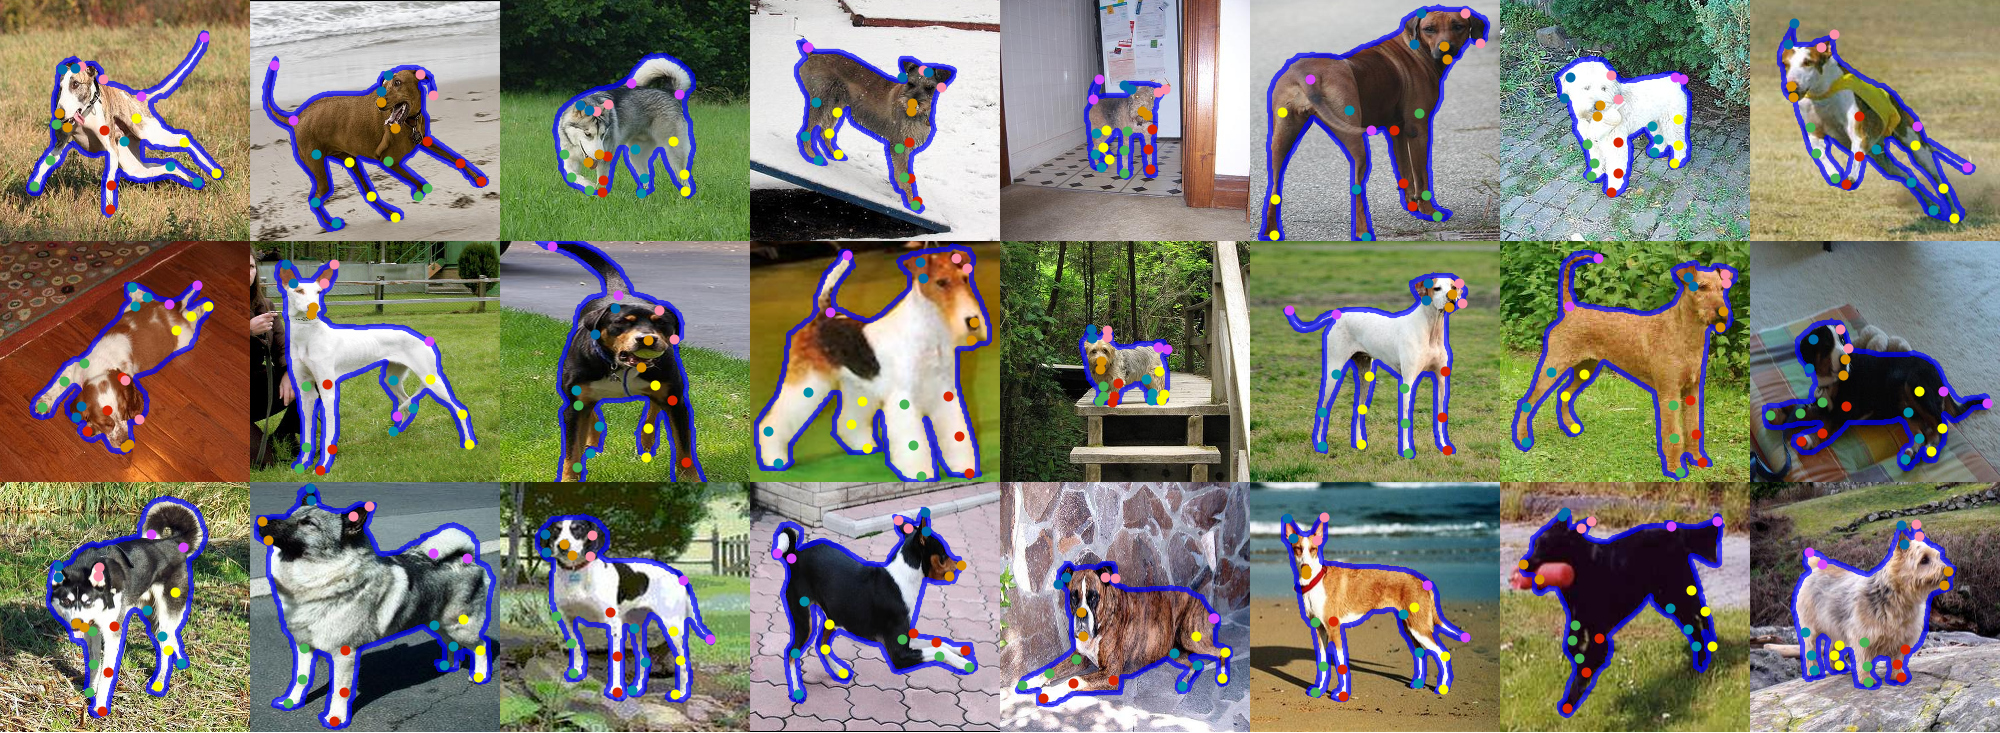
\includegraphics[height=0.1775\textheight]{OllieFigs/collage_wide.png}
    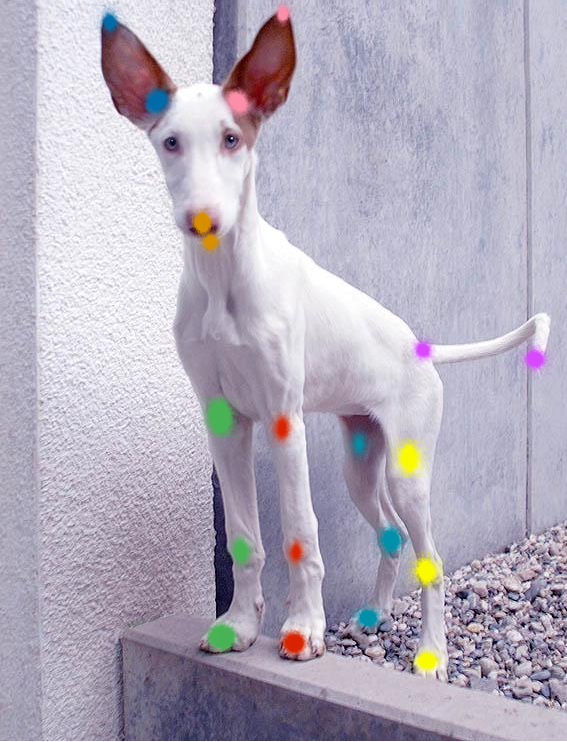
\includegraphics[height=0.1775\textheight]{OllieFigs/heatmap.png}
    \caption{\textbf{StanfordExtra example images}. \emph{Left}: outlined segmentations and labelled keypoints for 24 representative images. \emph{Right}: heatmap of deviation of worker submitted results from mean for each submission.}
    \label{fig:dataset}
\end{figure*}

In order to train and evaluate the method, it is neccessary to source a large-scale dataset of dog images with associated 2D annotations. This chapter therefore introduces \emph{StanfordExtra}: a new large-scale dataset with annotated 2D keypoints and binary segmentation masks for dogs. The source images were sourced from the existing Stanford Dog Dataset~\cite{StanfordDogs}, which consists of 20,580 dog images taken ``in the wild" and covers 120 dog breeds. The dataset contains vast shape and pose variation between dogs, as well as nuisance factors such as self/environmental occlusion, interaction with humans/other animals and partial views. Figure~\ref{fig:dataset} (left) shows samples from the new dataset.

Annotatations were collected using Amazon Mechanical Turk. The annotators (termed `turkers' on the platform) provided a binary silhouette mask and 20 keypoints per image. The remainder of this section describes the process for obtaining keypoint and segmentation annotations for the Stanford Dog Dataset~\cite{StanfordDogs}. 

The entire set of 20,580 dog images were first augmented with a single bounding box (provided with the original data) to indicate the largest dog in the image which the annotator should label. Each image was sent to 3 independent turkers with instructions explaining how to label the 20 keypoints and segmentation mask. 

\subsection{Keypoints.} 
Amazon turkers were given a list of 20 keypoints to click: 3 per leg (knee, ankle, toe), 2 per ear (base, tip), 2 per tail (base, tip), 2 per face (nose and jaw). They were additionally asked to provide a visibility flag per point. 

For each keypoint, we process the three clicks to yield a reliable coordinate. From the 3 clicks, we discard clicks that are further than a set tolerance from the mean. If at least 2 clicks remain, the mean coordinate is accepted as the keypoint position. Otherwise, the point has not been reliably identified so is set invisible. In line with other methods which tackle ``in-the-wild'' 3D reconstruction of articulated subjects~\cite{kolotouros19learning,kolotouros19convolutional}, images with fewer than a threshold number of visible keypoints (in this case 8 keypoints) are not included in StanfordExtra filtered from the dataset. This is since these images are unsuitable for the primary purpose of StanfordExtra, to train and evaluate full-body dog reconstruction task. 

% We rely on the following scheme to determine the optimal position of each keypoint, from the three annotations:

% \begin{enumerate}
%     \item 
% \end{enumerate}

% \begin{enumerate}
% \itemsep0em 
% \item{If If the keypoint was flagged highlighted by three different workers, and all three points are within a certain tolerance of the mean\footnote{Tolerance set at (Image width + Image height)/80, in pixels.}, then accept the mean as the keypoint position. If not, reject the furthest point from the mean, and go to step 2.}

% \item{If the keypoint was highlighted by two different workers, and both points are within a certain tolerance of the mean, accept the mean as the keypoint position. If not, reject the keypoint.}

% \item{If the keypoint was highlighted by only one worker, reject the keypoint.}

% \end{enumerate}


\subsection{Segmentation.}

\def\turker{t}
\def\turkertwo{t'}
\def\turkerboth{\bar{t}}

For each image, each worker $\turker \in \{\turker_{1}, \turker_{2}, \turker_{3}\}$ submits a binary segmentation mask $\mathbf{S}^{\turker}$. Submissions which fail simple criteria, such as if the segmentation area is below a threshold number of pixels, are sent for relabelling. 

% In order to sanitise the dataset and reduce erroneous entries, certain images were rejected or discarded. `Discarded' refers to a submission being discarded from the final dataset, whilst `rejected' means that the submission was deleted from the MTurk dataset, and a new entry requested from the website.\\

% As an initial pass, images were rejected (for which the bounding boxes were insufficiently large - to count null entries. For this, any entry was rejected if,

% \begin{equation}
% \sum\limits_{j=1}^H \sum\limits_{k=1}^W \mathbf{A}^{i,w}_{jk} < 0.01 WH 
% \end{equation}

For each image, the most likely segementation is generated by comparing submissions across workers. For any two turkers $\turker, \turkertwo$, a correlation coefficient is computed between submissions, summing over all pixels $i$. Note that $\bigotimes$ denotes the element-wise product of the matrices.

\begin{equation}
c(\turker, \turkertwo) = \frac{
    \sum_i \left[ \mathbf{S}^{\turker} \bigotimes \mathbf{S}^{\turkertwo} \right]_{i}}
    {\max\limits_{\turkerboth = \{\turker,\turkertwo\}} \sum_{i} \mathbf{S}^{\turkerboth}_{i}}
\end{equation}

% \begin{equation}
% c_{w,w'} = \frac{\mathbf{A}_{w} \odot \mathbf{A}_{w'}}{\max\limits_{p = \{w, w'\}}\mathbf{A}_{p}}
% \end{equation}

% We remove annotations for which all correlation coefficients are below 80\%. 
A worker's seggmentation $S^{\turker}$ is removed if all correlation coefficients $c(\turker,\turkertwo)$ are below a set threshold. The final binary mask is computed from the remaining submissions:

\begin{equation}
S^{*}_{i} = \begin{cases}
    1 & \text{if } \sum_{\turker} S^{\turker}_{i} > 1 \\
    0 & \text{otherwise}
\end{cases}
\end{equation}

\begin{figure}
\centering
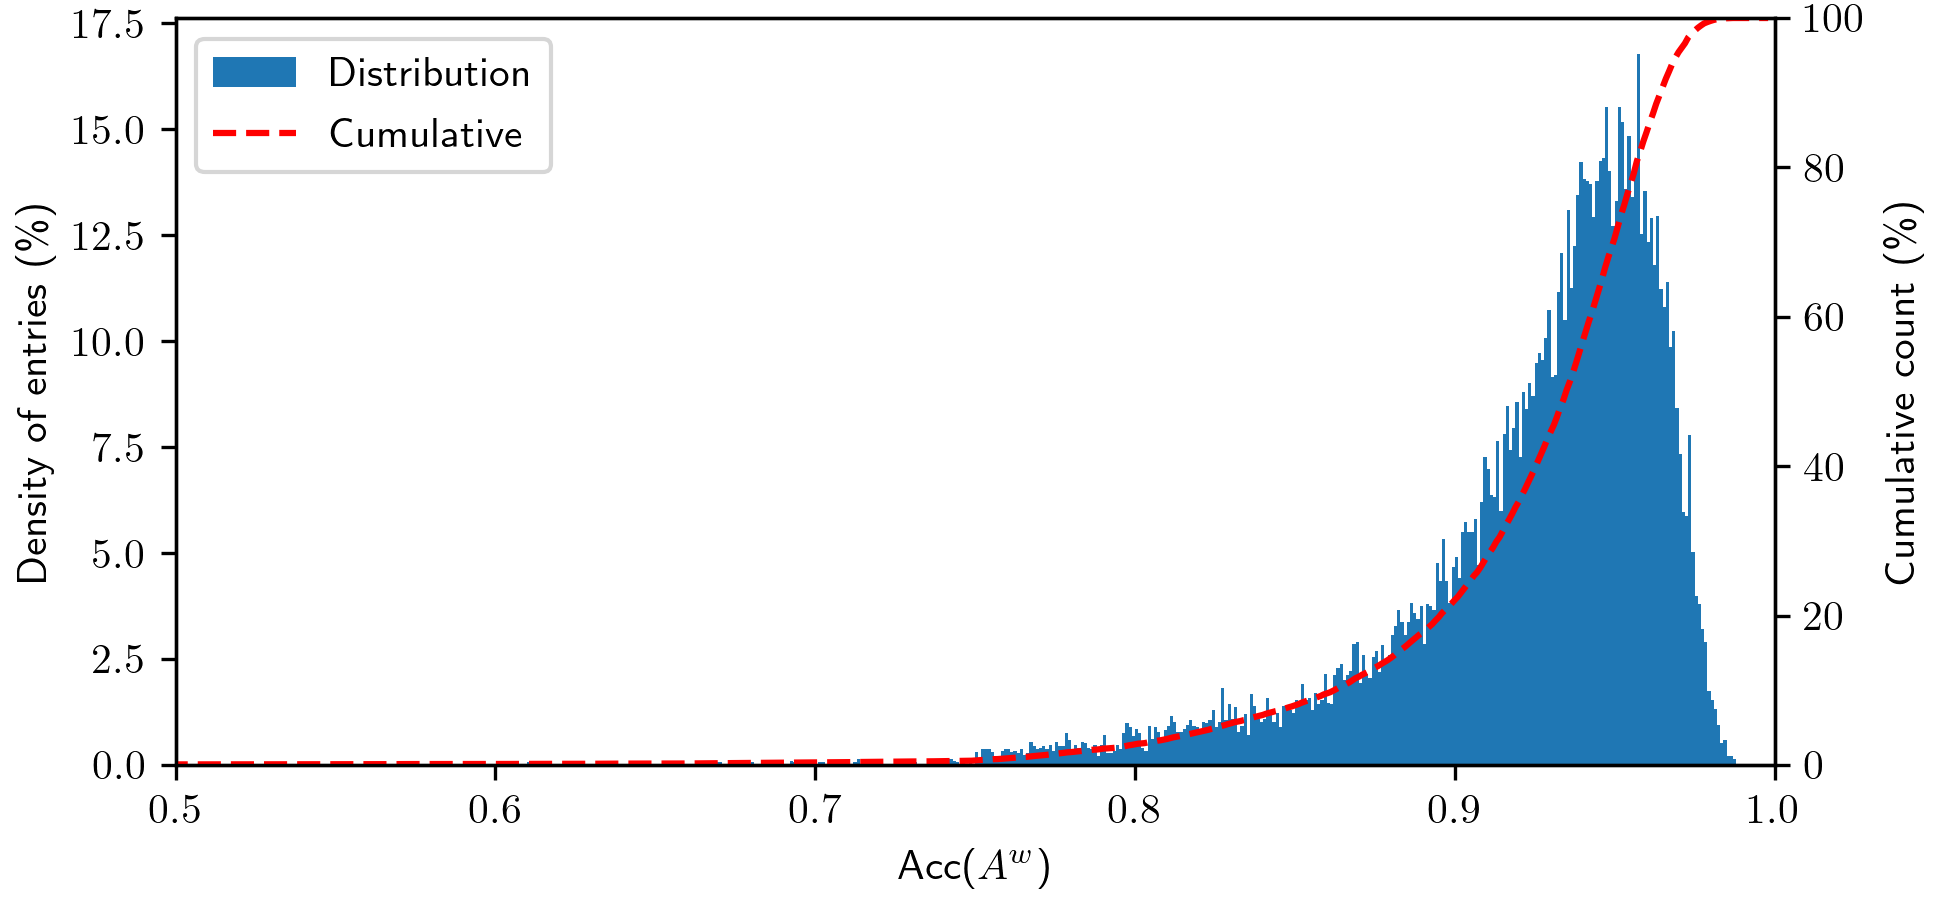
\includegraphics[width=0.95\textwidth]{OllieFigs/correlations.PNG}
\caption{Accuracy distribution of all submitted dog segmentations across the entire StanfordExtra dataset.}
\label{fig:accuracy distribution}
\end{figure}

With this, the accuracy of a worker's segmentation can be estimated according to the largest of their correlation coefficients: 

\begin{equation}
    \textrm{Acc}(S^{\turker})=\max_{\turkerboth \neq \turker} \{c(\turker, \turkerboth)\}
\end{equation}

\subsection{Approximating the dataset complexity.}

Figure~\ref{fig:dataset} gives an indication of the complexity of the dataset by analysing the distribution of worker accuracies across the entire StanfordExtra dataset.


% \subsubsection{Filtering the dataset.}

% As described in the paper, we reject images from our train/evaluation splits which based on reliability we deem unsuitable for our task of complete 3D reconstruction. have fewer than 8 identified keypoints find it necessary to reject The Stanford dog dataset contains 20,580 images. Not all of these images are constructive to this dataset - many do not have a lot of the dog in frame, etc. Several stages of refinement of the dataset were made, detailed in Table \ref{tab:filtering}.

% \begin{table}[]
%     \centering
%     \begin{tabular}{c|c}
%          \toprule
%          20,580 &  Stanford dataset\\
%          - (5,...) & Initial filtering based on bbox \\
%          - (5,...) & Images with fewer than 8 identified keypoints \\
%          - (60) & Images with insufficient segmentation accuracy \\
%          - (76) & Images for which more than one keypoint is outside of the segmentation\footnote{(with padding of 5 pixels)}\\
%          \midrule
%          9,647 & Final dataset\\
%          \bottomrule
%     \end{tabular}
%     \caption{Filtering process for final produced dataset}
%     \label{tab:filtering}
% \end{table}

\section{Experiments}

% As with other methods, we observe that introducing a silhouette term into the network loss before the model's pose has been somewhat solved can result in unsatisfactory local minima. We overcome this by using a pre-training stage with the following loss terms:


In this section, the WLDO method is compared against competitive baselines. The protocol for evaluation is described first, followed by a quantitative and qualitative evaluation.

\subsection{Evaluation protocol}

Evaluation is based on the StanfordExtra dataset introduced earlier in the chapter, which contains 8,476 images for 120 breeds. These images are divided per-breed into an 80\%/20\% train and test split.

Two primary evaluation metrics are considered. IoU is the intersection-over-union of the projected model silhouette compared to the ground truth annotation and indicates the quality of the reconstructed 3D shape. Percentage of Correct Keypoints (PCK) computes the percentage of joints which are within a normalized distance (based on square root of 2D silhouette area) to the ground truth locations, and evaluates the quality of reconstructed 3D pose. In addition, PCK results are produced for various joint groups (legs, tail, ears, face) in order to compare the reconstruction accuracy for different parts of the dog. Also used for evaluation is a new comparison metric \emph{PCK-MAX}. This protocol is similar to the Percentage of Correct Keypoints (PCK) metric~\cite{yang2013articulated} but incorporates the `invisible' ground-truth points. The standard PCK metric ignores these points, meaning even correct 3D reconstructions will receive no credit. PCK-MAX instead assumes reconstructed 3D points for missing ground-truth data are correct, providing an interesting upper bound.

\subsection{Training procedure}

The WLDO network is trained in two stages. The first omits the silhouette loss which tends to lead the network to unsatisfactory local minima if applied too early. With the silhouette loss turned off, it is satisfactory to use the simple unimodal prior (and without EM) for this preliminary stage since there is no loss to specifically encourage a strong shape alignment. After this, the silhouette loss and mixture prior with $M=10$ clusters are introduced, and expectation maximization updates are applied every 50 epochs. The first stage is trained for 250 epochs and the second stage for 150. The entire training procedure takes approximately 96 hours on a single P100 GPU.

Recall that the training objective for our end-to-end system for predicting SMBLD parameters consistent with a monocular dog input image is given by:

\begin{equation}
    \L{opt}=\L{joints}+\L{sil}+\L{pose}+\L{shape}+\L{mixture}
\end{equation}

Each loss term is weighted with a scalar $\W{}$. The following details the specific weights used for each training stage:

\ss{Stage 1.} $\W{joints}=10.0,\W{pose}=1.0,\W{shape}=1.0,\W{sil}=0.0,\W{mixture}=0.0$. This stage is trained for 250 epochs using the Adam optimizer, with learning rate set to $10^{-4}$. 
\ss{Stage 2.} $\W{joints}=10.0,\W{pose}=0.5,\W{shape}=0.0,\W{sil}=100.0,\W{mixture}=0.1$. This stage is trained for 150 epochs and run the described EM update step every $K=50$ epochs. The number of clusters $M=10$ was selected based on a grid search over $M=1,5,10,25$ with IoU scores compared. The Adam optimizer is again applied with learning rate to $10^{-5}$.

To begin, WLDO is compared with various baseline methods. 3D Menagerie (3D-M)~\cite{zuffi2017menagerie} is an approach which fits the 3D SMAL model using per-image energy minimization. Creatures Great and SMAL (CGAS)~\cite{biggs2018creatures} is a three-stage method, which employs a joint predictor on silhouette renderings from synthetic 3D dogs, applies a genetic algorithm to clean predictions, and finally applies the SMAL optimizer to produce the 3D mesh.

At test-time both 3D-M and CGAS rely on manually-provided segementation masks, and 3D-M also relies on hand-clicked keypoints. In order to produce a fair comparison, we produce a set of \emph{predicted} keypoints for StanfordExtra by training the Stacked Hourglass Network~\cite{newell2016stacked} with 8 stacks and 1 block, and \emph{predicted} segmentation masks using DeepLab v3+~\cite{deeplabv3plus}. The Stacked Hourglass Network achieves 71.4\% PCK score, DeepLab v3+ achieves 83.4\% IoU score and the CGAS joint predictor achieves 41.8\% PCK score. 

%All methods are trained from scratch and evaluated on our Stanford Dog validation set.

% \begin{table}[]
\centering
\begin{tabular}{@{}lcc@{}}
\toprule
\multicolumn{1}{l}{Method} & 
\multicolumn{1}{c}{IoU} & 
\multicolumn{1}{c}{PCK} 
\\ 
\midrule
DeepLab v3+ & 83.4 & --- \\
HourglassNet & --- & 71.4 \\
CGAS Joint Predictor & --- & 51.8 \\
\bottomrule 
\end{tabular}
\vspace{1em}
\caption{\label{tab:othernetworks}\textbf{Competitive Networks}. We evaluate the performance of Stacked Hourglass Network with 8 stacks and 1 block and DeepLab v3+ trained on our Stanford Dog training set and evaluated on the test set. We train CGAS on the synthetic data and evaluate on ground truth segmentations in the Stanford Dog test set.}
\end{table}
% \begin{table}[]
\centering
\begin{tabular}{@{}lcc@{}}
\toprule
\multicolumn{1}{l}{Method} & 
\multicolumn{1}{c}{IoU} & 
\multicolumn{1}{c}{PCK} 
\\ 
\midrule
DeepLab v3+ & 83.4 & --- \\
HourglassNet & --- & 71.4 \\
CGAS Joint Predictor & --- & 51.8 \\
\bottomrule 
\end{tabular}
\vspace{1em}
\caption{\label{tab:othernetworks}\textbf{Competitive Networks}. We evaluate the performance of Stacked Hourglass Network with 8 stacks and 1 block and DeepLab v3+ trained on our Stanford Dog training set and evaluated on the test set. We train CGAS on the synthetic data and evaluate on ground truth segmentations in the Stanford Dog test set.}
\end{table}

Table~\ref{tab:baselinesfix}, \Cref{fig:comparison_1} and \Cref{fig:comparison_2} show the comparison against competitive methods. For full examination, results for 3D-M and CGAS are additionally provided in the scenario that ground-truth keypoints and/or segmentations are available at test time. 

The results show our end-to-end method outperforms the competitors when they are provided with predicted keypoints/segmentations (white rows). The WLDO method therefore achieves a new state-of-the-art on this 3D reconstruction task. In addition, the method is shown to achieve improved average IoU/PCK scores than competitive methods, even when competitors are provided ground truth annotations at test time (grey rows). Also demonstrated is the wider applicability of two contributions of this chapter (scale parameters and improved prior) in the improved performance of the 3D-M method when these are incorporated. Finally, WLDO's test-time speed is significantly faster than competitive methods as no subsequent energy minimization procedure is required. 

\begin{table}[]
{
    \small
    \centering
    \begin{tabular}{@{}lcccccccc@{}}
    \toprule
    \multicolumn{1}{l}{Method} & 
    \multicolumn{1}{c}{Kps} & 
    \multicolumn{1}{c}{Seg} & 
    \multicolumn{1}{c}{IoU} & 
    \multicolumn{5}{c}{PCK @ 0.15} \\
    \multicolumn{4}{c}{} &
    \multicolumn{1}{c}{Avg} &
    \multicolumn{1}{c}{Legs} &
    \multicolumn{1}{c}{Tail} &
    \multicolumn{1}{c}{Ears} &
    \multicolumn{1}{c}{Face} \\
    \midrule
    \rowcolor{comp} 3D-M~\cite{zuffi2017menagerie} & Pred & Pred & 69.9 & 69.7 & 68.3 & 68.0 & 57.8 & 93.7 \\
    \rowcolor{notcomp} 3D-M & GT & GT & 71.0 & 75.6 & 74.2 & 89.5 & 60.7 & 98.6 \\
    \rowcolor{notcomp} 3D-M & GT & Pred & 70.7 & 75.5 & 74.1 & 88.1 & 60.2 & 98.7 \\
    \rowcolor{notcomp} 3D-M & Pred & GT & 70.5 & 70.3 & 69.0 & 69.4 & 58.5 & 94.0 \\
    \hline
    \rowcolor{comp} CGAS~\cite{biggs2018creatures} & CGAS & Pred & 63.5 & 28.6 & 30.7 & 34.5 & 25.9 & 24.1 \\
    \rowcolor{notcomp} CGAS & CGAS & GT & 64.2 & 28.2 & 30.1 & 33.4 & 26.3 & 24.5 \\
    \hline
    \rowcolor{comp} 3D-M + scaling & Pred & Pred & 70.4 & 70.9 & 69.8 & 66.9 & 59.7 & 94.0 \\
    \rowcolor{comp} 3D-M + scaling + EM prior & Pred & Pred & 71.8 & 73.4 & 72.5 & \textbf{70.3} & 62.6 & \textbf{94.1} \\
    \hline
    \rowcolor{comp} \textbf{Ours} & --- & --- & \textbf{74.2} & \textbf{78.8} & \textbf{76.4} & 63.9 & \textbf{78.1} & 92.1 \\
    \bottomrule 
    \end{tabular}
    \vspace{1em}
    \caption[]{\label{tab:baselinesfix}\textbf{Baseline comparisons.} PCK and silhouette IOU scores are shown for SOTA methods under varying conditions. Directly comparable baseline methods (requiring only an input image) are highlighted. \emph{Pred} keypoints generated with Hourglass-Net~\cite{newell2016stacked} and segmentations with DeepLab v3+~\cite{journals/corr/ChenPK0Y16}. 3D-M/CGAS are also analysed when they have access to ground-truth keypoints and/or segmentation masks. We also analyse adding this paper's innovations (scale parameters and EM prior) to 3D-M~\cite{zuffi2017menagerie}.}
}
\end{table}


\newcolumntype{?}{!{\vrule width 1pt}}

% \newcommand\sfac{0.082}
% \newcommand\spacercomp{4mm}
\begin{figure*}[ht!]
    \centering
    \setkeys{Gin}{width=\linewidth}
    \renewcommand\tabularxcolumn[1]{>{\Centering}m{\sfac\linewidth}} % set all columns to be centered v & hwise, with a fixed length
    \newcolumntype{D}{ >{\centering\arraybackslash} m{\imgwidthcomp} }
    \newcolumntype{E}{ >{\centering\arraybackslash} m{\labelwidthcomp} }

    % \begin{tabularx}{\textwidth}{c*{5}{X}@{\hspace{\spacercomp}}*{5}{X}c}
    % \begin{tabularx}{\textwidth}{c*{5}{X}}
    \begin{tabularx}{\textwidth}{EDDDDD}
      \textbf{Ours} &
      \includegraphics{ours_sup/n02086646-Blenheim_spaniel/orig/n02086646_1476.jpg} &
      \includegraphics{ours_sup/n02086646-Blenheim_spaniel/fit/n02086646_1476.jpg} &
      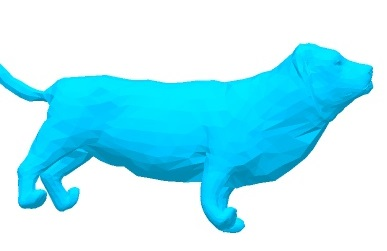
\includegraphics{ours_sup/n02086646-Blenheim_spaniel/model/n02086646_1476_crop.jpg} &
      \includegraphics{ours_sup/n02086646-Blenheim_spaniel/joints/n02086646_1476.jpg} &
      \includegraphics{ours_sup/n02086646-Blenheim_spaniel/segs/n02086646_1476.jpg} \\
      

      3D-M &
      \includegraphics{comp_sup/smal/n02086646-Blenheim_spaniel/orig/n02086646_1476.jpg} &
      \includegraphics{comp_sup/smal/n02086646-Blenheim_spaniel/fit/n02086646_1476.jpg} &
      \includegraphics{comp_sup/smal/n02086646-Blenheim_spaniel/model/n02086646_1476_fixed_crop.jpg} &
      \includegraphics{comp_sup/smal/n02086646-Blenheim_spaniel/joints/n02086646_1476.jpg} &
      \includegraphics{comp_sup/smal/n02086646-Blenheim_spaniel/segs/n02086646_1476.jpg} \\
      

      CGAS &
      \includegraphics{comp_sup/cgas/n02086646-Blenheim_spaniel/orig/n02086646_1476.jpg} &
      \includegraphics{comp_sup/cgas/n02086646-Blenheim_spaniel/fit/n02086646_1476.jpg} &
      \includegraphics{comp_sup/cgas/n02086646-Blenheim_spaniel/model/n02086646_1476_fixed_crop.jpg} &
      \includegraphics{comp_sup/cgas/n02086646-Blenheim_spaniel/joints/n02086646_1476.jpg} &
      \includegraphics{comp_sup/cgas/n02086646-Blenheim_spaniel/segs/n02086646_1476.jpg} \\
      %\hspace{\spacercomp}
     
      \textbf{Ours} &
      \includegraphics{ours_sup/n02087394-Rhodesian_ridgeback/orig/n02087394_831.jpg} &
      \includegraphics{ours_sup/n02087394-Rhodesian_ridgeback/fit/n02087394_831.jpg} &
      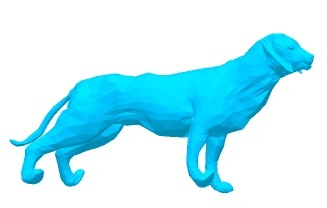
\includegraphics{ours_sup/n02087394-Rhodesian_ridgeback/model/n02087394_831_crop.jpg} &
      \includegraphics{ours_sup/n02087394-Rhodesian_ridgeback/joints/n02087394_831.jpg} &
      \includegraphics{ours_sup/n02087394-Rhodesian_ridgeback/segs/n02087394_831.jpg} \\

      3D-M &
      %\hspace{\spacercomp}
      \includegraphics{comp_sup/smal/n02087394-Rhodesian_ridgeback/orig/n02087394_831.jpg} &
      \includegraphics{comp_sup/smal/n02087394-Rhodesian_ridgeback/fit/n02087394_831.jpg} &
      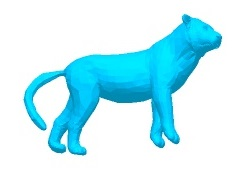
\includegraphics{comp_sup/smal/n02087394-Rhodesian_ridgeback/model/n02087394_831_fixed_crop.jpg} &
      \includegraphics{comp_sup/smal/n02087394-Rhodesian_ridgeback/joints/n02087394_831.jpg} &
      \includegraphics{comp_sup/smal/n02087394-Rhodesian_ridgeback/segs/n02087394_831.jpg} \\

      CGAS &
      \includegraphics{comp_sup/cgas/n02087394-Rhodesian_ridgeback/orig/n02087394_831.jpg} &
      \includegraphics{comp_sup/cgas/n02087394-Rhodesian_ridgeback/fit/n02087394_831.jpg} &
      \includegraphics{comp_sup/cgas/n02087394-Rhodesian_ridgeback/model/n02087394_831_fixed_crop.jpg} &
      \includegraphics{comp_sup/cgas/n02087394-Rhodesian_ridgeback/joints/n02087394_831.jpg} &
      \includegraphics{comp_sup/cgas/n02087394-Rhodesian_ridgeback/segs/n02087394_831.jpg} \\
      
      % & 
      & (a) & (b) & (c) & (d) & (e) \\
      %\hspace{\spacercomp} 
      % (a) & (b) & (c) & (d) & (e) \\
    \end{tabularx}
    %
    \caption{%
    \textbf{Qualitiative comparison to SOTA.} 
    Row 1: \textbf{Ours}, 
    Row 2: 3D-M~\cite{zuffi2017menagerie}, 
    Row 3: CGAS~\cite{biggs2018creatures}. 
    (a) input image, (b) predicted 3D mesh, (c) canonical view 3D mesh, 
    (d) reprojected model joints and (e) silhouette reprojection error. 
    }
    \label{fig:comparison_1}
\end{figure*}

\newcolumntype{?}{!{\vrule width 1pt}}

% \newcommand\sfac{0.082}
% \newcommand\spacercomp{4mm}
\begin{figure*}[ht!]
    \centering
    \setkeys{Gin}{width=\linewidth}
    \renewcommand\tabularxcolumn[1]{>{\Centering}m{\sfac\linewidth}} % set all columns to be centered v & hwise, with a fixed length
    \newcolumntype{D}{ >{\centering\arraybackslash} m{\imgwidthcomp} }
    \newcolumntype{E}{ >{\centering\arraybackslash} m{\labelwidthcomp} }

    % \begin{tabularx}{\textwidth}{c*{5}{X}@{\hspace{\spacercomp}}*{5}{X}c}
    % \begin{tabularx}{\textwidth}{c*{5}{X}}
    \begin{tabularx}{\textwidth}{EDDDDD}
      % \textbf{Ours} &
      % \includegraphics{ours_sup/n02086646-Blenheim_spaniel/orig/n02086646_1476.jpg} &
      % \includegraphics{ours_sup/n02086646-Blenheim_spaniel/fit/n02086646_1476.jpg} &
      % \includegraphics{ours_sup/n02086646-Blenheim_spaniel/model/n02086646_1476_crop.jpg} &
      % \includegraphics{ours_sup/n02086646-Blenheim_spaniel/joints/n02086646_1476.jpg} &
      % \includegraphics{ours_sup/n02086646-Blenheim_spaniel/segs/n02086646_1476.jpg} \\
      

      % 3D-M &
      % \includegraphics{comp_sup/smal/n02086646-Blenheim_spaniel/orig/n02086646_1476.jpg} &
      % \includegraphics{comp_sup/smal/n02086646-Blenheim_spaniel/fit/n02086646_1476.jpg} &
      % \includegraphics{comp_sup/smal/n02086646-Blenheim_spaniel/model/n02086646_1476_fixed_crop.jpg} &
      % \includegraphics{comp_sup/smal/n02086646-Blenheim_spaniel/joints/n02086646_1476.jpg} &
      % \includegraphics{comp_sup/smal/n02086646-Blenheim_spaniel/segs/n02086646_1476.jpg} \\
      

      % CGAS &
      % \includegraphics{comp_sup/cgas/n02086646-Blenheim_spaniel/orig/n02086646_1476.jpg} &
      % \includegraphics{comp_sup/cgas/n02086646-Blenheim_spaniel/fit/n02086646_1476.jpg} &
      % \includegraphics{comp_sup/cgas/n02086646-Blenheim_spaniel/model/n02086646_1476_fixed_crop.jpg} &
      % \includegraphics{comp_sup/cgas/n02086646-Blenheim_spaniel/joints/n02086646_1476.jpg} &
      % \includegraphics{comp_sup/cgas/n02086646-Blenheim_spaniel/segs/n02086646_1476.jpg} \\
      % %\hspace{\spacercomp}
     
      % \textbf{Ours} &
      % \includegraphics{ours_sup/n02087394-Rhodesian_ridgeback/orig/n02087394_831.jpg} &
      % \includegraphics{ours_sup/n02087394-Rhodesian_ridgeback/fit/n02087394_831.jpg} &
      % \includegraphics{ours_sup/n02087394-Rhodesian_ridgeback/model/n02087394_831_crop.jpg} &
      % \includegraphics{ours_sup/n02087394-Rhodesian_ridgeback/joints/n02087394_831.jpg} &
      % \includegraphics{ours_sup/n02087394-Rhodesian_ridgeback/segs/n02087394_831.jpg} \\

      % 3D-M &
      % %\hspace{\spacercomp}
      % \includegraphics{comp_sup/smal/n02087394-Rhodesian_ridgeback/orig/n02087394_831.jpg} &
      % \includegraphics{comp_sup/smal/n02087394-Rhodesian_ridgeback/fit/n02087394_831.jpg} &
      % \includegraphics{comp_sup/smal/n02087394-Rhodesian_ridgeback/model/n02087394_831_fixed_crop.jpg} &
      % \includegraphics{comp_sup/smal/n02087394-Rhodesian_ridgeback/joints/n02087394_831.jpg} &
      % \includegraphics{comp_sup/smal/n02087394-Rhodesian_ridgeback/segs/n02087394_831.jpg} \\

      % CGAS &
      % \includegraphics{comp_sup/cgas/n02087394-Rhodesian_ridgeback/orig/n02087394_831.jpg} &
      % \includegraphics{comp_sup/cgas/n02087394-Rhodesian_ridgeback/fit/n02087394_831.jpg} &
      % \includegraphics{comp_sup/cgas/n02087394-Rhodesian_ridgeback/model/n02087394_831_fixed_crop.jpg} &
      % \includegraphics{comp_sup/cgas/n02087394-Rhodesian_ridgeback/joints/n02087394_831.jpg} &
      % \includegraphics{comp_sup/cgas/n02087394-Rhodesian_ridgeback/segs/n02087394_831.jpg} \\
      
      \textbf{Ours} &
      \includegraphics{ours_sup/n02091134-whippet/orig/n02091134_16201.jpg} &
      \includegraphics{ours_sup/n02091134-whippet/fit/n02091134_16201.jpg} &
      \includegraphics{ours_sup/n02091134-whippet/model/n02091134_16201_crop.jpg} &
      \includegraphics{ours_sup/n02091134-whippet/joints/n02091134_16201.jpg} &
      \includegraphics{ours_sup/n02091134-whippet/segs/n02091134_16201.jpg} \\


      3D-M & 
      \includegraphics{comp_sup/smal/n02091134-whippet/orig/n02091134_16201.jpg} &
      \includegraphics{comp_sup/smal/n02091134-whippet/fit/n02091134_16201.jpg} &
      \includegraphics{comp_sup/smal/n02091134-whippet/model/n02091134_16201_fixed_crop.jpg} &
      \includegraphics{comp_sup/smal/n02091134-whippet/joints/n02091134_16201.jpg} &
      \includegraphics{comp_sup/smal/n02091134-whippet/segs/n02091134_16201.jpg} \\
      
      
      CGAS &
      \includegraphics{comp_sup/cgas/n02091134-whippet/orig/n02091134_16201.jpg} &
      \includegraphics{comp_sup/cgas/n02091134-whippet/fit/n02091134_16201.jpg} &
      \includegraphics{comp_sup/cgas/n02091134-whippet/model/n02091134_16201_fixed_crop.jpg} &
      \includegraphics{comp_sup/cgas/n02091134-whippet/joints/n02091134_16201.jpg} &
      \includegraphics{comp_sup/cgas/n02091134-whippet/segs/n02091134_16201.jpg} \\

      \textbf{Ours} &
      \includegraphics{ours_sup/n02089078-black-and-tan_coonhound/orig/n02089078_877.jpg} &
      \includegraphics{ours_sup/n02089078-black-and-tan_coonhound/fit/n02089078_877.jpg} &
      \includegraphics{ours_sup/n02089078-black-and-tan_coonhound/model/n02089078_877_crop.jpg} &
      \includegraphics{ours_sup/n02089078-black-and-tan_coonhound/joints/n02089078_877.jpg} &
      \includegraphics{ours_sup/n02089078-black-and-tan_coonhound/segs/n02089078_877.jpg} \\

      3D-M & 
      \includegraphics{comp_sup/smal/n02089078-black-and-tan_coonhound/orig/n02089078_877.jpg}&
      \includegraphics{comp_sup/smal/n02089078-black-and-tan_coonhound/fit/n02089078_877.jpg}&
      \includegraphics{comp_sup/smal/n02089078-black-and-tan_coonhound/model/n02089078_877_fixed_crop.jpg}&
      \includegraphics{comp_sup/smal/n02089078-black-and-tan_coonhound/joints/n02089078_877.jpg}&
      \includegraphics{comp_sup/smal/n02089078-black-and-tan_coonhound/segs/n02089078_877.jpg} \\
      
      CGAS &
      \includegraphics{comp_sup/cgas/n02089078-black-and-tan_coonhound/orig/n02089078_877.jpg}&
      \includegraphics{comp_sup/cgas/n02089078-black-and-tan_coonhound/fit/n02089078_877.jpg}&
      \includegraphics{comp_sup/cgas/n02089078-black-and-tan_coonhound/model/n02089078_877_fixed_crop.jpg}&
      \includegraphics{comp_sup/cgas/n02089078-black-and-tan_coonhound/joints/n02089078_877.jpg}&
      \includegraphics{comp_sup/cgas/n02089078-black-and-tan_coonhound/segs/n02089078_877.jpg} \\

      % \textbf{Ours} &
      % \includegraphics{ours_sup/n02087394-Rhodesian_ridgeback/orig/n02087394_831.jpg} &
      % \includegraphics{ours_sup/n02087394-Rhodesian_ridgeback/fit/n02087394_831.jpg} &
      % \includegraphics{ours_sup/n02087394-Rhodesian_ridgeback/model/n02087394_831.jpg} &
      % \includegraphics{ours_sup/n02087394-Rhodesian_ridgeback/joints/n02087394_831.jpg} &
      % \includegraphics{ours_sup/n02087394-Rhodesian_ridgeback/segs/n02087394_831.jpg} &
      % %\hspace{\spacercomp}


      % SMAL &
      % \includegraphics{comp_sup/smal/n02087394-Rhodesian_ridgeback/orig/n02087394_831.jpg} &
      % \includegraphics{comp_sup/smal/n02087394-Rhodesian_ridgeback/fit/n02087394_831.jpg} &
      % \includegraphics{comp_sup/smal/n02087394-Rhodesian_ridgeback/model/n02087394_831.jpg} &
      % \includegraphics{comp_sup/smal/n02087394-Rhodesian_ridgeback/joints/n02087394_831.jpg} &
      % \includegraphics{comp_sup/smal/n02087394-Rhodesian_ridgeback/segs/n02087394_831.jpg} &
      % %\hspace{\spacercomp}
      % \includegraphics{comp_sup/smal/n02089078-black-and-tan_coonhound/orig/n02089078_877.jpg} &
      % \includegraphics{comp_sup/smal/n02089078-black-and-tan_coonhound/fit/n02089078_877.jpg} &
      % \includegraphics{comp_sup/smal/n02089078-black-and-tan_coonhound/model/n02089078_877.jpg} &
      % \includegraphics{comp_sup/smal/n02089078-black-and-tan_coonhound/joints/n02089078_877.jpg} &
      % \includegraphics{comp_sup/smal/n02089078-black-and-tan_coonhound/segs/n02089078_877.jpg} \\

      % CGAS &
      % \includegraphics{comp_sup/cgas/n02087394-Rhodesian_ridgeback/orig/n02087394_831.jpg} &
      % \includegraphics{comp_sup/cgas/n02087394-Rhodesian_ridgeback/fit/n02087394_831.jpg} &
      % \includegraphics{comp_sup/cgas/n02087394-Rhodesian_ridgeback/model/n02087394_831.jpg} &
      % \includegraphics{comp_sup/cgas/n02087394-Rhodesian_ridgeback/joints/n02087394_831.jpg} &
      % \includegraphics{comp_sup/cgas/n02087394-Rhodesian_ridgeback/segs/n02087394_831.jpg} &
      % %\hspace{\spacercomp}
      % \includegraphics{comp_sup/cgas/n02089078-black-and-tan_coonhound/orig/n02089078_877.jpg} &
      % \includegraphics{comp_sup/cgas/n02089078-black-and-tan_coonhound/fit/n02089078_877.jpg} &
      % \includegraphics{comp_sup/cgas/n02089078-black-and-tan_coonhound/model/n02089078_877.jpg} &
      % \includegraphics{comp_sup/cgas/n02089078-black-and-tan_coonhound/joints/n02089078_877.jpg} &
      % \includegraphics{comp_sup/cgas/n02089078-black-and-tan_coonhound/segs/n02089078_877.jpg} \\

      % \textbf{Ours} &
      % \includegraphics{ours_sup/n02085936-Maltese_dog/orig/n02085936_3313.jpg} &
      % \includegraphics{ours_sup/n02085936-Maltese_dog/fit/n02085936_3313.jpg} &
      % \includegraphics{ours_sup/n02085936-Maltese_dog/model/n02085936_3313.jpg} &
      % \includegraphics{ours_sup/n02085936-Maltese_dog/joints/n02085936_3313.jpg} &
      % \includegraphics{ours_sup/n02085936-Maltese_dog/segs/n02085936_3313.jpg} &
      % %\hspace{\spacercomp}
      % \includegraphics{ours_sup/n02088238-basset/orig/n02088238_10054.jpg} &
      % \includegraphics{ours_sup/n02088238-basset/fit/n02088238_10054.jpg} &
      % \includegraphics{ours_sup/n02088238-basset/model/n02088238_10054.jpg} &
      % \includegraphics{ours_sup/n02088238-basset/joints/n02088238_10054.jpg} &
      % \includegraphics{ours_sup/n02088238-basset/segs/n02088238_10054.jpg} \\

      % SMAL &
      % \includegraphics{comp_sup/smal/n02085936-Maltese_dog/orig/n02085936_3313.jpg} &
      % \includegraphics{comp_sup/smal/n02085936-Maltese_dog/fit/n02085936_3313.jpg} &
      % \includegraphics{comp_sup/smal/n02085936-Maltese_dog/model/n02085936_3313.jpg} &
      % \includegraphics{comp_sup/smal/n02085936-Maltese_dog/joints/n02085936_3313.jpg} &
      % \includegraphics{comp_sup/smal/n02085936-Maltese_dog/segs/n02085936_3313.jpg} &
      % %\hspace{\spacercomp}
      % \includegraphics{comp_sup/smal/n02088238-basset/orig/n02088238_10054.jpg} &
      % \includegraphics{comp_sup/smal/n02088238-basset/fit/n02088238_10054.jpg} &
      % \includegraphics{comp_sup/smal/n02088238-basset/model/n02088238_10054.jpg} &
      % \includegraphics{comp_sup/smal/n02088238-basset/joints/n02088238_10054.jpg} &
      % \includegraphics{comp_sup/smal/n02088238-basset/segs/n02088238_10054.jpg} \\

      % CGAS &
      % \includegraphics{comp_sup/cgas/n02085936-Maltese_dog/orig/n02085936_3313.jpg} &
      % \includegraphics{comp_sup/cgas/n02085936-Maltese_dog/fit/n02085936_3313.jpg} &
      % \includegraphics{comp_sup/cgas/n02085936-Maltese_dog/model/n02085936_3313.jpg} &
      % \includegraphics{comp_sup/cgas/n02085936-Maltese_dog/joints/n02085936_3313.jpg} &
      % \includegraphics{comp_sup/cgas/n02085936-Maltese_dog/segs/n02085936_3313.jpg} &
      % %\hspace{\spacercomp}
      % \includegraphics{comp_sup/cgas/n02088238-basset/orig/n02088238_10054.jpg} &
      % \includegraphics{comp_sup/cgas/n02088238-basset/fit/n02088238_10054.jpg} &
      % \includegraphics{comp_sup/cgas/n02088238-basset/model/n02088238_10054.jpg} &
      % \includegraphics{comp_sup/cgas/n02088238-basset/joints/n02088238_10054.jpg} &
      % \includegraphics{comp_sup/cgas/n02088238-basset/segs/n02088238_10054.jpg} \\

      % & 
      & (a) & (b) & (c) & (d) & (e) \\
      %\hspace{\spacercomp} 
      % (a) & (b) & (c) & (d) & (e) \\
    \end{tabularx}
    %
    \caption{%
    \textbf{Qualitiative comparison to SOTA (continued).} 
    Row 1: \textbf{Ours}, 
    Row 2: 3D-M~\cite{zuffi2017menagerie}, 
    Row 3: CGAS~\cite{biggs2018creatures}. 
    (a) input image, (b) predicted 3D mesh, (c) canonical view 3D mesh, 
    (d) reprojected model joints and (e) silhouette reprojection error. 
    }
    \label{fig:comparison_2}
\end{figure*}


%xxx: Note that CGAS does badly as it can't clean up using video
\subsection{Generalization to unseen dataset}

Table~\ref{tab:animalposefix} shows an experiment to compare how well our model generalizes to a new data domain. We test our model against the 3D-M~\cite{zuffi2017menagerie} method (using predicted keypoints and segmentations as above for fairness) on the recent Animal Pose dataset~\cite{animalpose}. The data preparation process is the same as for StanfordExtra and no fine-tuning was used for either method. Good results are achieved in this unseen domain and still improve over the 3D-M optimizer.


\begin{table}
    \begin{tabular}{@{}lcccccc@{}}
    \toprule
    \multicolumn{1}{l}{Method} & 
    \multicolumn{1}{c}{IoU} & 
    \multicolumn{5}{c}{PCK @ 0.15} \\
    \multicolumn{2}{c}{} &
    \multicolumn{1}{c}{Avg} &
    \multicolumn{1}{c}{Legs} &
    \multicolumn{1}{c}{Tail} &
    \multicolumn{1}{c}{Ears} &
    \multicolumn{1}{c}{Face} \\
    \midrule
    3D-M~\cite{zuffi2017menagerie} & 64.9 & 59.2 & 55.7 & 56.9 & 61.3 & \textbf{86.7} \\
    % \hline
    \textbf{Ours} & \textbf{67.5} & \textbf{67.6} & \textbf{60.4} & \textbf{62.7} & \textbf{86.0} & \textbf{86.7} \\
    \bottomrule
    \end{tabular}
    \caption[]{
        \label{tab:animalposefix}
        \textbf{Animal Pose dataset~\cite{animalpose} results}. Evaluation on recent Animal Pose dataset with no fine-tuning to our method nor joint/silhouette predictors used for 3D-M.
    }
\end{table}


\begin{table}
    \begin{tabular}{@{}lcccccc@{}}
    \toprule
    \multicolumn{1}{l}{Method} & 
    \multicolumn{1}{c}{IoU} & 
    \multicolumn{5}{c}{PCK @ 0.1} \\
    \multicolumn{2}{c}{} &
    \multicolumn{1}{c}{Avg} &
    \multicolumn{1}{c}{Legs} &
    \multicolumn{1}{c}{Tail} &
    \multicolumn{1}{c}{Ears} &
    \multicolumn{1}{c}{Face} \\
    \midrule
    \textbf{Ours} & \textbf{74.2} & \textbf{63.7} & \textbf{59.5} & \textbf{48.1} & 60.1 & 88.0 \\
    $-$EM & 68.7 & 63.2 & 58.8 & 44.5 & \textbf{62.6} & 87.6 \\
    $-$MoG & 69.0 & 63.1 & \textbf{59.5} & 40.0 & 60.0 & \textbf{89.5} \\
    $-$Scale & 68.3 & 60.1 & 58.2 & 45.2 & 50.5 & 88.3 \\
    \bottomrule 
    \end{tabular}
    \caption[]{
        \label{tab:ablationfix}\textbf{Ablation study.} Evaluation with the following contributions removed: (a) EM updates, (b) Mixture Shape Prior, (c) SMBLD scale parameters.
    }
\end{table}


\subsection{Ablation study}

Secondly, an ablation of the individual components of the WLDO method is provided in order to examine the effect of each contribution on the PCK/IoU performance. Three variants are evaluated: (1) \textbf{Ours w/o EM} that omits EM updates, (2) \textbf{Ours w/o MoG} which replaces the mixture shape prior with a unimodal prior, (3)~\textbf{Ours w/o Scale} which removes the scale parameters. 

The results in Table~\ref{tab:ablationfix} indicate that each individual component has a positive impact on the overall method performance. In particular, it can be seen that the inclusion of the EM and Mixture of Gaussians prior leads to an improvement in IoU, suggesting that the shape prior refinements steps help the model accurately fit the exact dog shape. Interestingly, adding the Mixture of Gaussians prior but omitting EM steps slightly hinders performance, most likely due to an sub-optimal initialization for the $M$ clusters. However, adding EM updates to the Mixture of Gaussian model improves all metrics except the ear keypoint accuracy. It is observed that the error here is caused by the shape prior learning slightly imprecise shapes for dogs with extremely ``floppy'' ears. Although there is good silhouette coverage for these regions, the fact the SMBLD model has only a single articulation point per ear causes a lack of flexibility that results in occasionally misplaced ear tips for these instances. This could be improved in future work by adding additional model joints to the ear. Finally, the increased model flexibility afforded by the SMBLD scale parameters is shown to improve the IoU/PCK scores. 

\subsection{PCK-MAX results}

The final evaluation metric analyses PCK-MAX, a protocol which provides an upper bound on the PCK score by assuming invisible keypoints were successfully recovered.

\begin{table}[]
{
    \small
    \centering
    \begin{tabular}{@{}lcccccccc@{}}
    \toprule
    \multicolumn{1}{l}{Method} & 
    \multicolumn{1}{c}{Kps} & 
    \multicolumn{1}{c}{Seg} & 
    \multicolumn{5}{c}{PCK-MAX @ 0.1} \\
    \multicolumn{3}{c}{} &
    \multicolumn{1}{c}{Avg} &
    \multicolumn{1}{c}{Legs} &
    \multicolumn{1}{c}{Tail} &
    \multicolumn{1}{c}{Ears} &
    \multicolumn{1}{c}{Face} \\
    \midrule
    \rowcolor{comp} 3D-M~\cite{zuffi2017menagerie} & Pred & Pred & 67.1 & 65.7 & 79.5 & 54.9 & 87.4  \\
    \rowcolor{notcomp} 3D-M & GT & GT & 72.6 & 69.9 & 92.0 & 58.6 & 96.9 \\
    \rowcolor{notcomp} 3D-M & GT & Pred & 72.6 & 70.2 & 91.5 & 58.1 & 96.9 \\ 
    \rowcolor{notcomp} 3D-M & Pred & GT & 67.4 & 66.0 & 79.9 & 55.0 & 88.2 \\ 
    \hline
    \rowcolor{comp} CGAS~\cite{biggs2018creatures} & CGAS & Pred & 43.7 & 46.5 & 64.1 & 36.5 & 21.4  \\
    \rowcolor{notcomp} CGAS & CGAS & GT & 43.6 & 46.3 & 64.2 & 36.3 & 21.6 \\
    \hline
    \rowcolor{comp} 3D-M + scaling & Pred & Pred & 69.6 & 69.4 & 79.3 & 56.5 & 87.6 \\
    \rowcolor{comp} 3D-M + scaling + EM prior & Pred & Pred & 71.6 & 71.5 & \textbf{80.7} & 59.3 & 88.0 \\
    \hline
    \rowcolor{comp} \textbf{Ours} & --- & --- & \textbf{75.7} & \textbf{75.0} & 77.6 & \textbf{69.9} & \textbf{90.0} \\
    \bottomrule 
    \end{tabular}
    % \vspace{1em}
    \caption{\label{tab:baselines}\textbf{PCK-MAX baselines.} PCK-MAX scores are shown for SOTA methods under varying conditions. Directly comparable baseline methods (requiring only an input image) are highlighted. \emph{Pred} keypoints generated with Hourglass-Net~\cite{newell2016stacked} and segmentations with DeepLab v3+~\cite{journals/corr/ChenPK0Y16}. 3D-M/CGAS are also analysed when they have access to ground-truth keypoints and/or segmentation masks. We also analyse adding this paper's innovations (scale parameters and EM prior) to the 3D-M method~\cite{zuffi2017menagerie}.}
}
\end{table}
\begin{table}[!htbp]
    \begin{tabular}{@{}lccccc@{}}
    \toprule
    \multicolumn{1}{l}{Method} & 
    \multicolumn{5}{c}{PCK-MAX @ 0.1} \\
    \multicolumn{1}{c}{} &
    \multicolumn{1}{c}{Avg} &
    \multicolumn{1}{c}{Legs} &
    \multicolumn{1}{c}{Tail} &
    \multicolumn{1}{c}{Ears} &
    \multicolumn{1}{c}{Face} \\
    \midrule
    3D-M~\cite{zuffi2017menagerie} & 69.1 & 60.9 & 83.5 & 75.0 & 93.0 \\
    % \hline
    \textbf{Ours} & \textbf{73.8} & \textbf{65.1} & \textbf{85.6} & \textbf{84.0} & \textbf{93.6} \\
    \bottomrule
    % \multicolumn{6}{c}{} \\
    % \multicolumn{6}{c}{}
    % \textbf{Ours} & \textbf{66.9} & \textbf{73.8} & \textbf{65.1} & \textbf{85.6} & \textbf{84.0} & \textbf{93.6} \\
    % \textbf{Ours} & \textbf{66.9} & \textbf{73.8} & \textbf{65.1} & \textbf{85.6} & \textbf{84.0} & \textbf{93.6}
    \end{tabular}
    % \vspace{1em}
    \caption{
        \label{tab:animalpose}
        \textbf{PCK-MAX Animal Pose dataset~\cite{animalpose}}. Evaluation on recent Animal Pose dataset with no fine-tuning to our method nor joint/silhouette predictors used for 3D-M.}
\end{table}
    
\begin{table}[!htbp]
    \begin{tabular}{@{}lccccc@{}}
    \toprule
    \multicolumn{1}{l}{Method} & 
    \multicolumn{5}{c}{PCK-MAX @ 0.1} \\
    \multicolumn{1}{c}{} &
    \multicolumn{1}{c}{Avg} &
    \multicolumn{1}{c}{Legs} &
    \multicolumn{1}{c}{Tail} &
    \multicolumn{1}{c}{Ears} &
    \multicolumn{1}{c}{Face} \\
    \midrule
    \textbf{Ours} & \textbf{75.7} & \textbf{75.0} & \textbf{77.6} & 69.9 & 90.0 \\
    $-$EM & 74.6 & 72.9 & 75.2 & \textbf{72.5} & 88.3 \\
    $-$MoG & 74.9 & 74.3 & 73.3 & 70.0 & \textbf{90.2} \\ 
    $-$Scale & 72.6 & 72.9 & 75.3 & 62.3 & 89.1 \\
    \bottomrule 
    \end{tabular}
    % \vspace{1em}
    \caption{\label{tab:ablation}\textbf{PCK-MAX ablation study.} Evaluation with the following contributions removed: (a) EM updates, (b) Mixture Shape Prior, (c) SMBLD scale parameters.}
\end{table}



% \small
\centering
\begin{tabular}{@{}lllrrrr@{}}
\toprule
\multicolumn{1}{l}{Method} & 
\multicolumn{1}{c}{IoU} & 
\multicolumn{5}{c}{PCK} \\
\multicolumn{2}{c}{} &
\multicolumn{1}{c}{Avg} &
\multicolumn{1}{c}{Tail} &
\multicolumn{1}{c}{Ears} &
\multicolumn{1}{c}{Face} &
\multicolumn{1}{c}{Legs} \\
\midrule
Ours & \textbf{73.6} & \textbf{75.7} & \textbf{75.0} & \textbf{77.6} & 69.9 & 90.0 \\
Ours w/o EM & 67.7 & 74.6 & 72.9 & 75.2 & \textbf{72.5} & 88.3 \\
Ours w/o MoG & 68.0 & 74.9 & 74.3 & 73.3 & 70.0 & \textbf{90.2} \\ 
Ours w/o Scale & 67.3 & 72.6 & 72.9 & 75.3 & 62.3 & 89.1 \\
\bottomrule 
\end{tabular}
\vspace{1em}
\caption{\label{tab:ablation}\textbf{Ablation study.} Demonstration of how our methods perform when the following are removed: (a) Expectation Maximization updates, (b) Mixture Shape Prior, (c) Removing SMBLD scale parameters.}


% We are able to use the dataset to examine which dog parts are the most challenging to position. 
% \input{eccv2020kit/fig_jointspreads}
% \anote{TODO: PCK tables and errors visualized on 3D dog.}
% \paragraph{Analysis over breeds}
% A significant benefit of our dog dataset is that the supplied breed labels allows for reconstruction performance to be evaluated over particular breeds. \anote{Figure} ranks the breeds by error.
% \begin{table}[]
\small
\centering
\begin{tabular}{@{}lrrrr@{}}
\toprule
\multicolumn{1}{l}{} & 
\multicolumn{1}{c}{PCK}         & 
\multicolumn{1}{c}{IoU}         & 
\multicolumn{1}{c}{Metric 3}         & 
\multicolumn{1}{c}{Metric 4}          
\\ \midrule
\multicolumn{1}{r}{Daschund}             & 109.1                    & 99.6                     & 96.5                     & 95.5                     \\

\end{tabular}
\vspace{1em}
\caption{\label{tab:breed}\textbf{Evaluation of breeds} showing that there is a difference}
\end{table}

\subsection{Qualitative evaluation}

Figures \ref{fig:qualresults_se_1}, \ref{fig:qualresults_se_2} and \ref{fig:qualresults_se_3} shows a range of example system outputs when tested on range of StanfordExtra dogs with varying pose and shape and in challenging conditions. Figure \ref{fig:qualresults_ani} shows results on the Animal Pose dataset. Note that only StanfordExtra is used for training.


% \input{fig_comparison}

% \input{fig_qualresults}

% \input{fig_qual_results_animal_pose}
% \section{Failure Cases}

% \footnotetext[4]{PCK results in tables have been updated to match definitions of Yang and Ramanan~\cite{yang2013articulated} normalized by 2D silhouette area. Please see original tables and further details in the appendix.}


\section{Conclusions}
This paper presents an end-to-end method for automatic, monocular 3D dog reconstruction. This is achieved using only weak 2D supervision, provided by the StanfordExtra dataset which has been introduced in this chapter. Further, it has been shown that a more detailed shape prior can be learned by tuning a gaussian mixture during model training and this leads to improved reconstructions. In addition, the WLDO method improves over competitive baselines, even when they are given access to ground truth data at test time.

Future work should involve tackling some failure cases of our system, for example handling multiple overlapping dogs or dealing with heavy motion blur. Other areas for research include extending the EM formulation introduced here to handle video input to take advantage of multi-view shape constraints. Finally, an interesting direction may be to transfer knowledge accumulated through training on StanfordExtra dogs to enable accurate 3D shape reconstruction for other species.

% \newcolumntype{?}{!{\vrule width 1pt}}

\newcolumntype{M}[1]{>{\centering\arraybackslash}m{#1}}
\newcommand\scalefactorqual{0.085}
\newcommand\spacerqual{3mm}

\begin{figure*}[t!]
    \centering
    \setkeys{Gin}{width=\linewidth}
    %M{40pt}
    \renewcommand\tabularxcolumn[1]{>{\Centering}m{\scalefactorqual\linewidth}} % set all columns to be centered v & hwise, with a fixed width
    % \begin{tabularx}{\textwidth}{m{15pt}*{5}{X} @ {\hspace{\spacerqual}}*{5}{X}}%
    \begin{tabularx}{\textwidth}{m{15pt}*{5}{X}}
    
        %260pt = 8 rows, 
        \multirow{-2}{*}{\rotatebox[origin=c]{90}{$\overbrace{\hspace{293pt}}^{\textrm{\large StanfordExtra}}$}} &
    
        % R1
        \includegraphics{ours_sup/n02093256-Staffordshire_bullterrier/orig/n02093256_5791.jpg} &
        \includegraphics{ours_sup/n02093256-Staffordshire_bullterrier/fit/n02093256_5791.jpg} &
        \includegraphics{ours_sup/n02093256-Staffordshire_bullterrier/model/n02093256_5791_crop.jpg} &
        \includegraphics{ours_sup/n02093256-Staffordshire_bullterrier/joints/n02093256_5791.jpg} &
        \includegraphics{ours_sup/n02093256-Staffordshire_bullterrier/segs/n02093256_5791.jpg} \\
        %\hspace{\spacercomp} 
        &\includegraphics{ours_sup/n02088364-beagle/orig/n02088364_2499.jpg} & 
        \includegraphics{ours_sup/n02088364-beagle/fit/n02088364_2499.jpg} & 
        \includegraphics{ours_sup/n02088364-beagle/model/n02088364_2499_crop.jpg} & 
        \includegraphics{ours_sup/n02088364-beagle/joints/n02088364_2499.jpg} & 
        \includegraphics{ours_sup/n02088364-beagle/segs/n02088364_2499.jpg} \\ 

        % R2
        &\includegraphics{ours_sup/n02107908-Appenzeller/orig/n02107908_933.jpg} & 
        \includegraphics{ours_sup/n02107908-Appenzeller/fit/n02107908_933.jpg} & 
        \includegraphics{ours_sup/n02107908-Appenzeller/model/n02107908_933.jpg} & 
        \includegraphics{ours_sup/n02107908-Appenzeller/joints/n02107908_933.jpg} & 
        \includegraphics{ours_sup/n02107908-Appenzeller/segs/n02107908_933.jpg} \\
        %\hspace{\spacercomp} 
        &\includegraphics{ours_sup/n02088094-Afghan_hound/orig/n02088094_1917.jpg} & 
        \includegraphics{ours_sup/n02088094-Afghan_hound/fit/n02088094_1917.jpg} & 
        \includegraphics{ours_sup/n02088094-Afghan_hound/model/n02088094_1917.jpg} & 
        \includegraphics{ours_sup/n02088094-Afghan_hound/joints/n02088094_1917.jpg} & 
        \includegraphics{ours_sup/n02088094-Afghan_hound/segs/n02088094_1917.jpg} \\ 

        % R3
        &\includegraphics{ours_sup/n02087394-Rhodesian_ridgeback/orig/n02087394_7056.jpg} & 
        \includegraphics{ours_sup/n02087394-Rhodesian_ridgeback/fit/n02087394_7056.jpg} & 
        \includegraphics{ours_sup/n02087394-Rhodesian_ridgeback/model/n02087394_7056_crop.jpg} & 
        \includegraphics{ours_sup/n02087394-Rhodesian_ridgeback/joints/n02087394_7056.jpg} & 
        \includegraphics{ours_sup/n02087394-Rhodesian_ridgeback/segs/n02087394_7056.jpg} \\
        %\hspace{\spacercomp} 
        &\includegraphics{ours_sup/n02099601-golden_retriever/orig/n02099601_304.jpg} & 
        \includegraphics{ours_sup/n02099601-golden_retriever/fit/n02099601_304.jpg} & 
        \includegraphics{ours_sup/n02099601-golden_retriever/model/n02099601_304_crop.jpg} & 
        \includegraphics{ours_sup/n02099601-golden_retriever/joints/n02099601_304.jpg} & 
        \includegraphics{ours_sup/n02099601-golden_retriever/segs/n02099601_304.jpg} \\ 
        
        % R4
        &\includegraphics{ours_sup/n02085620-Chihuahua/orig/n02085620_3651.jpg} & 
        \includegraphics{ours_sup/n02085620-Chihuahua/fit/n02085620_3651.jpg} & 
        \includegraphics{ours_sup/n02085620-Chihuahua/model/n02085620_3651_crop.jpg} &
        \includegraphics{ours_sup/n02085620-Chihuahua/joints/n02085620_3651.jpg} &
        \includegraphics{ours_sup/n02085620-Chihuahua/segs/n02085620_3651.jpg} \\
        %\hspace{\spacercomp} 
        % \includegraphics{ours_sup/n02091134-whippet/orig/n02091134_16201.jpg} &
        % \includegraphics{ours_sup/n02091134-whippet/fit/n02091134_16201.jpg} &
        % \includegraphics{ours_sup/n02091134-whippet/model/n02091134_16201.jpg} &
        % \includegraphics{ours_sup/n02091134-whippet/joints/n02091134_16201.jpg} &
        % \includegraphics{ours_sup/n02091134-whippet/segs/n02091134_16201.jpg} \\ 
        &\includegraphics{ours_sup/n02097130-giant_schnauzer/orig/n02097130_5121.jpg} &
        \includegraphics{ours_sup/n02097130-giant_schnauzer/fit/n02097130_5121.jpg} &
        \includegraphics{ours_sup/n02097130-giant_schnauzer/model/n02097130_5121_crop.jpg} &
        \includegraphics{ours_sup/n02097130-giant_schnauzer/joints/n02097130_5121.jpg} &
        \includegraphics{ours_sup/n02097130-giant_schnauzer/segs/n02097130_5121.jpg} \\
        
        % R5
        &\includegraphics{ours_sup/n02089078-black-and-tan_coonhound/orig/n02089078_877.jpg} &
        \includegraphics{ours_sup/n02089078-black-and-tan_coonhound/fit/n02089078_877.jpg} &
        \includegraphics{ours_sup/n02089078-black-and-tan_coonhound/model/n02089078_877_crop.jpg} &
        \includegraphics{ours_sup/n02089078-black-and-tan_coonhound/joints/n02089078_877.jpg} &
        \includegraphics{ours_sup/n02089078-black-and-tan_coonhound/segs/n02089078_877.jpg} \\
        %\hspace{\spacercomp} 
        &\includegraphics{ours_sup/n02085620-Chihuahua/orig/n02085620_1152.jpg} &
        \includegraphics{ours_sup/n02085620-Chihuahua/fit/n02085620_1152.jpg} &
        \includegraphics{ours_sup/n02085620-Chihuahua/model/n02085620_1152_crop.jpg} &
        \includegraphics{ours_sup/n02085620-Chihuahua/joints/n02085620_1152.jpg} &
        \includegraphics{ours_sup/n02085620-Chihuahua/segs/n02085620_1152.jpg} \\ 
        
        % R6
        &\includegraphics{ours_sup/n02108000-EntleBucher/orig/n02108000_3104.jpg} &
        \includegraphics{ours_sup/n02108000-EntleBucher/fit/n02108000_3104.jpg} &
        \includegraphics{ours_sup/n02108000-EntleBucher/model/n02108000_3104_crop.jpg} &
        \includegraphics{ours_sup/n02108000-EntleBucher/joints/n02108000_3104.jpg} &
        \includegraphics{ours_sup/n02108000-EntleBucher/segs/n02108000_3104.jpg} \\
        %\hspace{\spacercomp} 
        &\includegraphics{ours_sup/n02105162-malinois/orig/n02105162_688.jpg} &
        \includegraphics{ours_sup/n02105162-malinois/fit/n02105162_688.jpg} &
        \includegraphics{ours_sup/n02105162-malinois/model/n02105162_688_crop.jpg} &
        \includegraphics{ours_sup/n02105162-malinois/joints/n02105162_688.jpg} &
        \includegraphics{ours_sup/n02105162-malinois/segs/n02105162_688.jpg} \\ 
        
        % R7
        &\includegraphics{ours_sup/n02102318-cocker_spaniel/orig/n02102318_11648.jpg} &
        \includegraphics{ours_sup/n02102318-cocker_spaniel/fit/n02102318_11648.jpg} &
        \includegraphics{ours_sup/n02102318-cocker_spaniel/model/n02102318_11648_crop.jpg} &
        \includegraphics{ours_sup/n02102318-cocker_spaniel/joints/n02102318_11648.jpg} &
        \includegraphics{ours_sup/n02102318-cocker_spaniel/segs/n02102318_11648.jpg} \\
        %\hspace{\spacercomp}
        &\includegraphics{ours_sup/n02086910-papillon/orig/n02086910_3020.jpg} &
        \includegraphics{ours_sup/n02086910-papillon/fit/n02086910_3020.jpg} &
        \includegraphics{ours_sup/n02086910-papillon/model/n02086910_3020_crop.jpg} &
        \includegraphics{ours_sup/n02086910-papillon/joints/n02086910_3020.jpg} &
        \includegraphics{ours_sup/n02086910-papillon/segs/n02086910_3020.jpg} \\
        
        % R8
        % &\includegraphics{ours_sup/n02097130-giant_schnauzer/orig/n02097130_5121.jpg} &
        % \includegraphics{ours_sup/n02097130-giant_schnauzer/fit/n02097130_5121.jpg} &
        % \includegraphics{ours_sup/n02097130-giant_schnauzer/model/n02097130_5121.jpg} &
        % \includegraphics{ours_sup/n02097130-giant_schnauzer/joints/n02097130_5121.jpg} &
        % \includegraphics{ours_sup/n02097130-giant_schnauzer/segs/n02097130_5121.jpg} &
        % \hspace{\spacercomp} 
        % \includegraphics{ours_sup/n02087394-Rhodesian_ridgeback/orig/n02087394_831.jpg} &
        % \includegraphics{ours_sup/n02087394-Rhodesian_ridgeback/fit/n02087394_831.jpg} &
        % \includegraphics{ours_sup/n02087394-Rhodesian_ridgeback/model/n02087394_831.jpg} &
        % \includegraphics{ours_sup/n02087394-Rhodesian_ridgeback/joints/n02087394_831.jpg} &
        % \includegraphics{ours_sup/n02087394-Rhodesian_ridgeback/segs/n02087394_831.jpg} \\

        % R9
        &\includegraphics{ours_sup/n02091032-Italian_greyhound/orig/n02091032_1933.jpg} &
        \includegraphics{ours_sup/n02091032-Italian_greyhound/fit/n02091032_1933.jpg} &
        \includegraphics{ours_sup/n02091032-Italian_greyhound/model/n02091032_1933_crop.jpg} &
        \includegraphics{ours_sup/n02091032-Italian_greyhound/joints/n02091032_1933.jpg} &
        \includegraphics{ours_sup/n02091032-Italian_greyhound/segs/n02091032_1933.jpg} \\
        %\hspace{\spacercomp}
        &\includegraphics{ours_sup/n02093647-Bedlington_terrier/orig/n02093647_3594.jpg} &
        \includegraphics{ours_sup/n02093647-Bedlington_terrier/fit/n02093647_3594.jpg} &
        \includegraphics{ours_sup/n02093647-Bedlington_terrier/model/n02093647_3594_crop.jpg} &
        \includegraphics{ours_sup/n02093647-Bedlington_terrier/joints/n02093647_3594.jpg} &
        \includegraphics{ours_sup/n02093647-Bedlington_terrier/segs/n02093647_3594.jpg} \\

        %R10
        &\includegraphics{ours_sup/n02106662-German_shepherd/orig/n02106662_13599.jpg} &
        \includegraphics{ours_sup/n02106662-German_shepherd/fit/n02106662_13599.jpg} &
        \includegraphics{ours_sup/n02106662-German_shepherd/model/n02106662_13599_crop.jpg} &
        \includegraphics{ours_sup/n02106662-German_shepherd/joints/n02106662_13599.jpg} &
        \includegraphics{ours_sup/n02106662-German_shepherd/segs/n02106662_13599.jpg} \\
        %\hspace{\spacercomp} 
        &\includegraphics{ours_sup/n02095314-wire-haired_fox_terrier/orig/n02095314_261.jpg} &
        \includegraphics{ours_sup/n02095314-wire-haired_fox_terrier/fit/n02095314_261.jpg} &
        \includegraphics{ours_sup/n02095314-wire-haired_fox_terrier/model/n02095314_261.jpg} &
        \includegraphics{ours_sup/n02095314-wire-haired_fox_terrier/joints/n02095314_261.jpg} &
        \includegraphics{ours_sup/n02095314-wire-haired_fox_terrier/segs/n02095314_261.jpg} \\

        % R11
        \multirow{-2.1}{*}{\rotatebox[origin=c]{90}{$\overbrace{\hspace{64pt}}^{\textrm{\large Animal Pose}}$}} &
        
        \includegraphics{ours_sup/animal_pose_fits/orig/2007_000063.jpg} &
        \includegraphics{ours_sup/animal_pose_fits/fit/2007_000063.jpg} &
        \includegraphics{ours_sup/animal_pose_fits/model/2007_000063_crop.jpg} &
        \includegraphics{ours_sup/animal_pose_fits/joints/2007_000063.jpg} &
        \includegraphics{ours_sup/animal_pose_fits/segs/2007_000063.jpg} \\
        %\hspace{\spacercomp} 
        &\includegraphics{ours_sup/animal_pose_fits/orig/2007_004189.jpg} &
        \includegraphics{ours_sup/animal_pose_fits/fit/2007_004189.jpg} &
        \includegraphics{ours_sup/animal_pose_fits/model/2007_004189_crop.jpg} &
        \includegraphics{ours_sup/animal_pose_fits/joints/2007_004189.jpg} &
        \includegraphics{ours_sup/animal_pose_fits/segs/2007_004189.jpg} \\ 

        % R12
        &\includegraphics{ours_sup/animal_pose_fits/orig/2007_008222.jpg} &
        \includegraphics{ours_sup/animal_pose_fits/fit/2007_008222.jpg} &
        \includegraphics{ours_sup/animal_pose_fits/model/2007_008222_crop.jpg} &
        \includegraphics{ours_sup/animal_pose_fits/joints/2007_008222.jpg} &
        \includegraphics{ours_sup/animal_pose_fits/segs/2007_008222.jpg} \\
        %\hspace{\spacercomp} 
        \includegraphics{ours_sup/animal_pose_fits/orig/2007_009605.jpg} &
        \includegraphics{ours_sup/animal_pose_fits/fit/2007_009605.jpg} &
        \includegraphics{ours_sup/animal_pose_fits/model/2007_009605_crop.jpg} &
        \includegraphics{ours_sup/animal_pose_fits/joints/2007_009605.jpg} &
        \includegraphics{ours_sup/animal_pose_fits/segs/2007_009605.jpg} \\ 
        
        & (a) & (b) & (c) & (d) & (e) \\
        %\hspace{\spacercomp} 
        % (a) & (b) & (c) & (d) & (e) \\

    \end{tabularx}
    %
    \caption{%
    \textbf{Qualitative results on StanfordExtra and Animal Pose~\cite{animalpose}.} 
        For each sample we show: (a) input image, (b) predicted 3D mesh, 
        (c) canonical view 3D mesh, (d) reprojected model joints and 
        (e) silhouette reprojection error.
    }
    \label{fig:qualresults_sup}
\end{figure*}


\newcolumntype{?}{!{\vrule width 1pt}}

% \newcolumntype{M}[1]{>{\centering\arraybackslash}m{#1}}
% \newcommand\scalefactorqual{0.085}
% \newcommand\spacerqual{3mm}

\begin{figure*}[t!]
    \centering
    \setkeys{Gin}{width=\linewidth}
    %M{40pt}
    \renewcommand\tabularxcolumn[1]{>{\Centering}m{\sfacqual\linewidth}} % set all columns to be centered v & hwise, with a fixed width
    % \begin{tabularx}{\textwidth}{m{15pt}*{5}{X} @ {\hspace{\spacerqual}}*{5}{X}}%
    % \begin{tabularx}{\textwidth}{m{15pt}*{5}{X}}
    \begin{tabularx}{\textwidth}{m{50pt}*{5}{X}}
    
        % %260pt = 8 rows, 
        % \multirow{-2}{*}{\rotatebox[origin=c]{90}{$\overbrace{\hspace{293pt}}^{\textrm{\large StanfordExtra}}$}} &
    
        % R1
        \includegraphics{ours_sup/n02093256-Staffordshire_bullterrier/orig/n02093256_5791.jpg} &
        \includegraphics{ours_sup/n02093256-Staffordshire_bullterrier/fit/n02093256_5791.jpg} &
        \includegraphics{ours_sup/n02093256-Staffordshire_bullterrier/model/n02093256_5791_crop.jpg} &
        \includegraphics{ours_sup/n02093256-Staffordshire_bullterrier/joints/n02093256_5791.jpg} &
        \includegraphics{ours_sup/n02093256-Staffordshire_bullterrier/segs/n02093256_5791.jpg} \\
        %\hspace{\spacercomp} 
        \includegraphics{ours_sup/n02088364-beagle/orig/n02088364_2499.jpg} & 
        \includegraphics{ours_sup/n02088364-beagle/fit/n02088364_2499.jpg} & 
        \includegraphics{ours_sup/n02088364-beagle/model/n02088364_2499_crop.jpg} & 
        \includegraphics{ours_sup/n02088364-beagle/joints/n02088364_2499.jpg} & 
        \includegraphics{ours_sup/n02088364-beagle/segs/n02088364_2499.jpg} \\ 

        % R2
        \includegraphics{ours_sup/n02107908-Appenzeller/orig/n02107908_933.jpg} & 
        \includegraphics{ours_sup/n02107908-Appenzeller/fit/n02107908_933.jpg} & 
        \includegraphics{ours_sup/n02107908-Appenzeller/model/n02107908_933.jpg} & 
        \includegraphics{ours_sup/n02107908-Appenzeller/joints/n02107908_933.jpg} & 
        \includegraphics{ours_sup/n02107908-Appenzeller/segs/n02107908_933.jpg} \\
        %\hspace{\spacercomp} 
        \includegraphics{ours_sup/n02088094-Afghan_hound/orig/n02088094_1917.jpg} & 
        \includegraphics{ours_sup/n02088094-Afghan_hound/fit/n02088094_1917.jpg} & 
        \includegraphics{ours_sup/n02088094-Afghan_hound/model/n02088094_1917.jpg} & 
        \includegraphics{ours_sup/n02088094-Afghan_hound/joints/n02088094_1917.jpg} & 
        \includegraphics{ours_sup/n02088094-Afghan_hound/segs/n02088094_1917.jpg} \\ 

        % R3
        \includegraphics{ours_sup/n02087394-Rhodesian_ridgeback/orig/n02087394_7056.jpg} & 
        \includegraphics{ours_sup/n02087394-Rhodesian_ridgeback/fit/n02087394_7056.jpg} & 
        \includegraphics{ours_sup/n02087394-Rhodesian_ridgeback/model/n02087394_7056_crop.jpg} & 
        \includegraphics{ours_sup/n02087394-Rhodesian_ridgeback/joints/n02087394_7056.jpg} & 
        \includegraphics{ours_sup/n02087394-Rhodesian_ridgeback/segs/n02087394_7056.jpg} \\
        %\hspace{\spacercomp} 
        \includegraphics{ours_sup/n02099601-golden_retriever/orig/n02099601_304.jpg} & 
        \includegraphics{ours_sup/n02099601-golden_retriever/fit/n02099601_304.jpg} & 
        \includegraphics{ours_sup/n02099601-golden_retriever/model/n02099601_304_crop.jpg} & 
        \includegraphics{ours_sup/n02099601-golden_retriever/joints/n02099601_304.jpg} & 
        \includegraphics{ours_sup/n02099601-golden_retriever/segs/n02099601_304.jpg} \\ 
        
        % R4
        \includegraphics{ours_sup/n02085620-Chihuahua/orig/n02085620_3651.jpg} & 
        \includegraphics{ours_sup/n02085620-Chihuahua/fit/n02085620_3651.jpg} & 
        \includegraphics{ours_sup/n02085620-Chihuahua/model/n02085620_3651_crop.jpg} &
        \includegraphics{ours_sup/n02085620-Chihuahua/joints/n02085620_3651.jpg} &
        \includegraphics{ours_sup/n02085620-Chihuahua/segs/n02085620_3651.jpg} \\
        %\hspace{\spacercomp} 
        % \includegraphics{ours_sup/n02091134-whippet/orig/n02091134_16201.jpg} &
        % \includegraphics{ours_sup/n02091134-whippet/fit/n02091134_16201.jpg} &
        % \includegraphics{ours_sup/n02091134-whippet/model/n02091134_16201.jpg} &
        % \includegraphics{ours_sup/n02091134-whippet/joints/n02091134_16201.jpg} &
        % \includegraphics{ours_sup/n02091134-whippet/segs/n02091134_16201.jpg} \\ 
        \includegraphics{ours_sup/n02097130-giant_schnauzer/orig/n02097130_5121.jpg} &
        \includegraphics{ours_sup/n02097130-giant_schnauzer/fit/n02097130_5121.jpg} &
        \includegraphics{ours_sup/n02097130-giant_schnauzer/model/n02097130_5121_crop.jpg} &
        \includegraphics{ours_sup/n02097130-giant_schnauzer/joints/n02097130_5121.jpg} &
        \includegraphics{ours_sup/n02097130-giant_schnauzer/segs/n02097130_5121.jpg} \\
        
        % R5
        \includegraphics{ours_sup/n02089078-black-and-tan_coonhound/orig/n02089078_877.jpg} &
        \includegraphics{ours_sup/n02089078-black-and-tan_coonhound/fit/n02089078_877.jpg} &
        \includegraphics{ours_sup/n02089078-black-and-tan_coonhound/model/n02089078_877_crop.jpg} &
        \includegraphics{ours_sup/n02089078-black-and-tan_coonhound/joints/n02089078_877.jpg} &
        \includegraphics{ours_sup/n02089078-black-and-tan_coonhound/segs/n02089078_877.jpg} \\
        %\hspace{\spacercomp} 
        \includegraphics{ours_sup/n02085620-Chihuahua/orig/n02085620_1152.jpg} &
        \includegraphics{ours_sup/n02085620-Chihuahua/fit/n02085620_1152.jpg} &
        \includegraphics{ours_sup/n02085620-Chihuahua/model/n02085620_1152_crop.jpg} &
        \includegraphics{ours_sup/n02085620-Chihuahua/joints/n02085620_1152.jpg} &
        \includegraphics{ours_sup/n02085620-Chihuahua/segs/n02085620_1152.jpg} \\ 
        
        % R6
        \includegraphics{ours_sup/n02108000-EntleBucher/orig/n02108000_3104.jpg} &
        \includegraphics{ours_sup/n02108000-EntleBucher/fit/n02108000_3104.jpg} &
        \includegraphics{ours_sup/n02108000-EntleBucher/model/n02108000_3104_crop.jpg} &
        \includegraphics{ours_sup/n02108000-EntleBucher/joints/n02108000_3104.jpg} &
        \includegraphics{ours_sup/n02108000-EntleBucher/segs/n02108000_3104.jpg} \\
        %\hspace{\spacercomp} 
        \includegraphics{ours_sup/n02105162-malinois/orig/n02105162_688.jpg} &
        \includegraphics{ours_sup/n02105162-malinois/fit/n02105162_688.jpg} &
        \includegraphics{ours_sup/n02105162-malinois/model/n02105162_688_crop.jpg} &
        \includegraphics{ours_sup/n02105162-malinois/joints/n02105162_688.jpg} &
        \includegraphics{ours_sup/n02105162-malinois/segs/n02105162_688.jpg} \\ 
        
        % R7
        \includegraphics{ours_sup/n02102318-cocker_spaniel/orig/n02102318_11648.jpg} &
        \includegraphics{ours_sup/n02102318-cocker_spaniel/fit/n02102318_11648.jpg} &
        \includegraphics{ours_sup/n02102318-cocker_spaniel/model/n02102318_11648_crop.jpg} &
        \includegraphics{ours_sup/n02102318-cocker_spaniel/joints/n02102318_11648.jpg} &
        \includegraphics{ours_sup/n02102318-cocker_spaniel/segs/n02102318_11648.jpg} \\
        %\hspace{\spacercomp}
        \includegraphics{ours_sup/n02086910-papillon/orig/n02086910_3020.jpg} &
        \includegraphics{ours_sup/n02086910-papillon/fit/n02086910_3020.jpg} &
        \includegraphics{ours_sup/n02086910-papillon/model/n02086910_3020_crop.jpg} &
        \includegraphics{ours_sup/n02086910-papillon/joints/n02086910_3020.jpg} &
        \includegraphics{ours_sup/n02086910-papillon/segs/n02086910_3020.jpg} \\
        
        % R8
        % &\includegraphics{ours_sup/n02097130-giant_schnauzer/orig/n02097130_5121.jpg} &
        % \includegraphics{ours_sup/n02097130-giant_schnauzer/fit/n02097130_5121.jpg} &
        % \includegraphics{ours_sup/n02097130-giant_schnauzer/model/n02097130_5121.jpg} &
        % \includegraphics{ours_sup/n02097130-giant_schnauzer/joints/n02097130_5121.jpg} &
        % \includegraphics{ours_sup/n02097130-giant_schnauzer/segs/n02097130_5121.jpg} &
        % \hspace{\spacercomp} 
        % \includegraphics{ours_sup/n02087394-Rhodesian_ridgeback/orig/n02087394_831.jpg} &
        % \includegraphics{ours_sup/n02087394-Rhodesian_ridgeback/fit/n02087394_831.jpg} &
        % \includegraphics{ours_sup/n02087394-Rhodesian_ridgeback/model/n02087394_831.jpg} &
        % \includegraphics{ours_sup/n02087394-Rhodesian_ridgeback/joints/n02087394_831.jpg} &
        % \includegraphics{ours_sup/n02087394-Rhodesian_ridgeback/segs/n02087394_831.jpg} \\

        % R9
        \includegraphics{ours_sup/n02091032-Italian_greyhound/orig/n02091032_1933.jpg} &
        \includegraphics{ours_sup/n02091032-Italian_greyhound/fit/n02091032_1933.jpg} &
        \includegraphics{ours_sup/n02091032-Italian_greyhound/model/n02091032_1933_crop.jpg} &
        \includegraphics{ours_sup/n02091032-Italian_greyhound/joints/n02091032_1933.jpg} &
        \includegraphics{ours_sup/n02091032-Italian_greyhound/segs/n02091032_1933.jpg} \\
        %\hspace{\spacercomp}
        \includegraphics{ours_sup/n02093647-Bedlington_terrier/orig/n02093647_3594.jpg} &
        \includegraphics{ours_sup/n02093647-Bedlington_terrier/fit/n02093647_3594.jpg} &
        \includegraphics{ours_sup/n02093647-Bedlington_terrier/model/n02093647_3594_crop.jpg} &
        \includegraphics{ours_sup/n02093647-Bedlington_terrier/joints/n02093647_3594.jpg} &
        \includegraphics{ours_sup/n02093647-Bedlington_terrier/segs/n02093647_3594.jpg} \\

        %R10
        \includegraphics{ours_sup/n02106662-German_shepherd/orig/n02106662_13599.jpg} &
        \includegraphics{ours_sup/n02106662-German_shepherd/fit/n02106662_13599.jpg} &
        \includegraphics{ours_sup/n02106662-German_shepherd/model/n02106662_13599_crop.jpg} &
        \includegraphics{ours_sup/n02106662-German_shepherd/joints/n02106662_13599.jpg} &
        \includegraphics{ours_sup/n02106662-German_shepherd/segs/n02106662_13599.jpg} \\
        %\hspace{\spacercomp} 
        \includegraphics{ours_sup/n02095314-wire-haired_fox_terrier/orig/n02095314_261.jpg} &
        \includegraphics{ours_sup/n02095314-wire-haired_fox_terrier/fit/n02095314_261.jpg} &
        \includegraphics{ours_sup/n02095314-wire-haired_fox_terrier/model/n02095314_261.jpg} &
        \includegraphics{ours_sup/n02095314-wire-haired_fox_terrier/joints/n02095314_261.jpg} &
        \includegraphics{ours_sup/n02095314-wire-haired_fox_terrier/segs/n02095314_261.jpg} \\

        (a) & (b) & (c) & (d) & (e) \\
        %\hspace{\spacercomp} 
        % (a) & (b) & (c) & (d) & (e) \\

    \end{tabularx}
    %
    \caption{%
    \textbf{Qualitative results on StanfordExtra and Animal Pose~\cite{animalpose}.} 
        For each sample we show: (a) input image, (b) predicted 3D mesh, 
        (c) canonical view 3D mesh, (d) reprojected model joints and 
        (e) silhouette reprojection error.
    }
    \label{fig:qualresults_sup}
\end{figure*}

\newcolumntype{?}{!{\vrule width 1pt}}

% \newcolumntype{M}[1]{>{\centering\arraybackslash}m{#1}}
% \newcommand\scalefactorqual{0.085}
% \newcommand\spacerqual{3mm}

\begin{figure*}[t!]
    \centering
    \setkeys{Gin}{width=\linewidth}
    \renewcommand\tabularxcolumn[1]{>{\Centering}m{\sfac\linewidth}} % set all columns to be centered v & hwise, with a fixed width
    % \begin{tabularx}{\textwidth}{m{15pt}*{5}{X} @ {\hspace{\spacerqual}}*{5}{X}}%
    % \begin{tabularx}{\textwidth}{m{15pt}*{5}{X}}
    \begin{tabularx}{\textwidth}{m{50pt}*{5}{X}}
        
    \includegraphics{ours_sup/animal_pose_fits/orig/2007_000063.jpg} &
    \includegraphics{ours_sup/animal_pose_fits/fit/2007_000063.jpg} &
    \includegraphics{ours_sup/animal_pose_fits/model/2007_000063_crop.jpg} &
    \includegraphics{ours_sup/animal_pose_fits/joints/2007_000063.jpg} &
    \includegraphics{ours_sup/animal_pose_fits/segs/2007_000063.jpg} \\
    %\hspace{\spacercomp} 
    \includegraphics{ours_sup/animal_pose_fits/orig/2007_004189.jpg} &
    \includegraphics{ours_sup/animal_pose_fits/fit/2007_004189.jpg} &
    \includegraphics{ours_sup/animal_pose_fits/model/2007_004189_crop.jpg} &
    \includegraphics{ours_sup/animal_pose_fits/joints/2007_004189.jpg} &
    \includegraphics{ours_sup/animal_pose_fits/segs/2007_004189.jpg} \\ 

    % R12
    \includegraphics{ours_sup/animal_pose_fits/orig/2007_008222.jpg} &
    \includegraphics{ours_sup/animal_pose_fits/fit/2007_008222.jpg} &
    \includegraphics{ours_sup/animal_pose_fits/model/2007_008222_crop.jpg} &
    \includegraphics{ours_sup/animal_pose_fits/joints/2007_008222.jpg} &
    \includegraphics{ours_sup/animal_pose_fits/segs/2007_008222.jpg} \\
    %\hspace{\spacercomp} 
    \includegraphics{ours_sup/animal_pose_fits/orig/2007_009605.jpg} &
    \includegraphics{ours_sup/animal_pose_fits/fit/2007_009605.jpg} &
    \includegraphics{ours_sup/animal_pose_fits/model/2007_009605_crop.jpg} &
    \includegraphics{ours_sup/animal_pose_fits/joints/2007_009605.jpg} &
    \includegraphics{ours_sup/animal_pose_fits/segs/2007_009605.jpg} \\ 
    
    (a) & (b) & (c) & (d) & (e) \\
        %\hspace{\spacercomp} 
        % (a) & (b) & (c) & (d) & (e) \\

    \end{tabularx}
    %
    \caption{%
    \textbf{Qualitative results on StanfordExtra and Animal Pose~\cite{animalpose}.} 
        For each sample we show: (a) input image, (b) predicted 3D mesh, 
        (c) canonical view 3D mesh, (d) reprojected model joints and 
        (e) silhouette reprojection error.
    }
    \label{fig:qualresults_sup}
\end{figure*}



